\RequirePackage{fix-cm}
\documentclass[11pt,a4paper]{article}
\usepackage{cmap}
\usepackage[T1]{fontenc}
\usepackage[sc]{mathpazo}
\linespread{1.04}
\DeclareFontShape{T1}{cmtt}{bx}{n}{<->ssub*cmtt/m/n}{}
\usepackage{colortbl}
\usepackage[margin=2.4cm]{geometry}
\usepackage{amsmath,amssymb,amsthm,mathtools}
\usepackage{booktabs,longtable,array,tabularx}
\usepackage{pdflscape}
\usepackage{enumitem}
\usepackage{xcolor}
\usepackage{tikz}
\usetikzlibrary{arrows.meta,positioning,calc,shapes.geometric,fit,backgrounds,decorations.pathreplacing}
\usepackage{pgfplots}
\pgfplotsset{compat=1.16}
\usepackage[final]{microtype}
\usepackage[colorlinks=true,linkcolor=blue!50!black,citecolor=blue!50!black,urlcolor=blue!50!black]{hyperref}
\usepackage[capitalise]{cleveref}

\definecolor{accA}{HTML}{1F5E8C}
\definecolor{accB}{HTML}{8C4A1F}
\definecolor{accC}{HTML}{2E7D4F}
\definecolor{lvE}{HTML}{E8F1F8}
\definecolor{lvT}{HTML}{F1EEF8}
\definecolor{lvO}{HTML}{FBEFE6}

\newtheorem{theorem}{Theorem}
\newtheorem{corollary}{Corollary}
\newtheorem{proposition}{Proposition}
\theoremstyle{definition}
\newtheorem{definition}{Definition}
\newtheorem{example}{Example}
\theoremstyle{remark}
\newtheorem{remark}{Remark}

\newcommand{\Dstruct}{D_{\mathrm{struct}}}
\newcommand{\dstruct}{d_{\mathrm{struct}}}
\newcommand{\dspec}{d_{\mathrm{spec}}}
\newcommand{\AYM}{\mathcal{A}_{\mathrm{YM}}}
\newcommand{\SUNNS}{\mathcal{S}_{\mathrm{UNNS}}}
\newcommand{\Yspec}{\mathcal{Y}_{\mathrm{spec}}}
\newcommand{\Pset}{\mathcal{P}}
\newcommand{\sqs}{\sqrt{\sigma}}
\newcommand{\uns}{UNNS}
\newcommand{\Hacc}{\mathrm{H}_{\mathrm{acc}}}
\newcommand{\Hiso}{\mathrm{H}_{\mathrm{iso}}}
\setlist{itemsep=2pt,topsep=4pt}
\setlength{\parindent}{1.2em}
\setlength{\emergencystretch}{2em}
\renewcommand{\arraystretch}{1.12}

\title{\textbf{Structural Accessibility and Spectral Discreteness in Pure SU(3) Yang--Mills:}\\[2pt]
\large A \uns{} Reassessment of Vacuum Non-Crossability and the Mass Gap}
\author{UNNS Substrate Project}
\date{October 2026}

\begin{document}
\maketitle

\begin{abstract}
\noindent We investigate whether the Yang--Mills mass gap requires a structurally non-crossable neighborhood around the vacuum. An initial \uns{} non-crossability program distinguishes massive from gapless controls but fails to establish a universal refinement-stable vacuum boundary. We then test the alternative hypothesis that the Yang--Mills vacuum is structurally accessible within the same admissible domain. Across connected chromoelectric-field profiles, common-refinement analysis, canonical \uns{} structural chambers, an unsmoothed connected-correlator control, and a vacuum-subtracted continuum energy--momentum-tensor representation, no universal positive structural exclusion floor is detected. Independent continuum glueball spectroscopy nevertheless retains a strictly positive scalar excitation scale. The combined result supports the coexistence of structural vacuum accessibility with spectral discreteness and therefore separates structural proximity to the vacuum from spectral proximity to the vacuum.

\smallskip\noindent On the mathematical side, we prove a \emph{structural--spectral separation theorem}. A positive spectral gap does not by itself imply a structural exclusion neighborhood; continuity of the excitation-energy functional at the vacuum provides a sufficient bridge to such an exclusion, while structural accessibility under a persistent gap forces that continuity to fail. The theorem is elementary---it is essentially continuity---and we say so; its role is to locate the missing assumption of the original program. We separate throughout an \emph{empirical} accessibility statement, which the frozen evidence supports, from a \emph{limit} statement, which it does not establish. The substantive open problem is the specialization to Yang--Mills: constructing the structure-to-spectrum map $\Pi:\SUNNS\to\Yspec$ and determining its topology. We do not prove $V\in\overline{\AYM}$, and nothing here addresses the Clay mass-gap problem.
\end{abstract}

\vspace{2pt}
\noindent\textbf{Keywords:} Yang--Mills mass gap; glueball spectrum; UNNS; structural accessibility; spectral gap; common refinement; falsifiability.

\setcounter{tocdepth}{1}\tableofcontents
\newpage

%==============================================================
\section{Introduction: does a mass gap require a structural gap?}\label{sec:intro}

The Yang--Mills mass gap is a statement about the Hamiltonian spectrum: the lowest excited eigenvalue lies strictly above the vacuum energy, $E_1-E_0>0$. The \uns{} (Unbounded Nested Number Sequences) program studies recursion-generated structure, and one natural question within it is whether this spectral separation has a \emph{structural} shadow---whether the vacuum sits behind a wall in structure space that every non-vacuum admissible configuration must respect. This paper reports the outcome of testing that idea in two successive, fully frozen research projects, and extracts from the outcome a precise mathematical statement about what such a wall would and would not follow from.

The first project, \texttt{UNNS\_YM\_GAP}, asked whether the mass gap corresponds to a refinement-stable structural non-crossability boundary. It built an explicit diagnostic, tested it against deliberately constructed gapless adversaries, and followed it through model and measured-data refinement. The idea was not established, and the closing evidence was uncertainty-limited rather than decisive. The second project, \texttt{UNNS\_VACUUM\_CONTINUITY}, then asked the converse question: is the vacuum structurally accessible, and can that accessibility coexist with an independently retained spectral scale? Its answer, within a frozen evidence architecture, is yes. Taken together the two projects are not two reports but one argument with a correction in the middle, and this paper presents them that way.

\subsection{Four notions of nearness}
The phrase ``close to the vacuum'' hides several distinct notions, and the paper is organized around keeping them apart.
\begin{itemize}
\item \emph{Configuration-space nearness}: a gauge-field configuration close to the trivial one in some norm.
\item \emph{Observable-space nearness}: a gauge-invariant profile (a field strength, a correlator, an energy--momentum-tensor component) whose vacuum-subtracted contrast is small. This is what the structural chambers of the two projects actually measure; we write $\dstruct$ or $\Dstruct$ for such distances.
\item \emph{Hilbert-space nearness}: a state vector close to the vacuum vector in norm.
\item \emph{Spectral nearness}: $\dspec(E_n,E_0)=E_n-E_0$, a property of Hamiltonian eigenvalues.
\end{itemize}
Nothing forces these to share a topology. The original hypothesis implicitly identified the second with the fourth; \cref{sec:theorem} shows exactly what that identification would require, and \cref{sec:discussion} returns to the four notions.

\subsection{Hypotheses: isolation, empirical accessibility, limit accessibility}
Let $\AYM$ be the admissible Yang--Mills-derived structural domain, $V$ the vacuum object, and $\Dstruct$ a structural distance. The first project tested the \emph{isolation} (non-crossability) hypothesis,
\begin{equation}\label{eq:Hiso}
\Hiso:\qquad \Dstruct(X,V)\;\ge\;\delta>0\quad\text{for all admissible non-vacuum }X,\ \text{stably under refinement.}
\end{equation}
The second project replaced it by accessibility. The word ``accessibility'' is used in two strengths, and the distinction is central:
\begin{align}
\Hacc^{\mathrm{emp}}:&\quad\text{in the tested representations no universal positive exclusion floor is detected and}\notag\\
&\quad\text{structural vacuum accessibility is supported, while a positive spectral scale is retained;}\label{eq:Hemp}\\
\Hacc^{\mathrm{lim}}:&\quad\exists\,X_n\in\AYM\setminus\{V\}:\ \Dstruct(X_n,V)\to0\quad\text{while}\quad E_1-E_0>0.\label{eq:Hlim}
\end{align}
\Cref{eq:Hemp} is a statement about the outcome of frozen experiments; \cref{eq:Hlim} is a mathematical limit statement about a sequence in a representation-independent metric. The projects support the first and do not establish the second:
\begin{equation}\label{eq:status}
\boxed{\ \Hiso\ \text{is not established};\qquad \Hacc^{\mathrm{emp}}\ \text{is supported};\qquad \Hacc^{\mathrm{lim}}\ \text{is not yet established.}\ }
\end{equation}
In particular the Stage-2 ``structural states'' are spatial profile windows and ladders of vacuum-subtracted observables, not excitation sequences carrying an energy functional (\cref{rem:premise}).

\subsection{Contributions, in three levels}
We keep three levels of statement strictly separate; the whole manuscript is organized around the separation.
\begin{center}
\renewcommand{\arraystretch}{1.25}
\begin{tabular}{@{}>{\columncolor{lvE}\raggedright\arraybackslash}p{4.3cm}>{\columncolor{lvT}\raggedright\arraybackslash}p{5.2cm}>{\columncolor{lvO}\raggedright\arraybackslash}p{5.2cm}@{}}
\textbf{Level 1: Empirical result} & \textbf{Level 2: Elementary theorem} & \textbf{Level 3: Open \uns{} theorem problem}\\
Structural accessibility is supported ($\Hacc^{\rm emp}$) and coexists with a positive spectral scale in the tested pure-SU(3) representations (\cref{sec:stage2,sec:stage3,sec:bridge}). &
A spectral gap implies structural exclusion only under a continuity/coercivity bridge; accessibility plus a gap forces that bridge to fail (\cref{sec:theorem}). &
Construct the structure-to-spectrum map $\Pi:\SUNNS\to\Yspec$ and determine its topology (\cref{sec:implications}).
\end{tabular}
\end{center}

\begin{figure}[t]
\centering
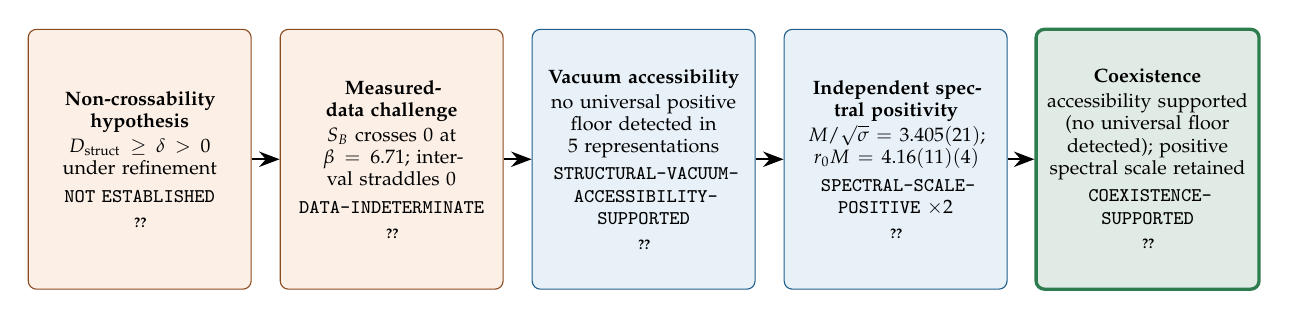
\begin{tikzpicture}[
 bx/.style={draw=accA,fill=lvE,rounded corners=3pt,text width=2.55cm,align=center,inner sep=4pt,font=\scriptsize,minimum height=3.3cm},
 hy/.style={draw=accB,fill=lvO,rounded corners=3pt,text width=2.55cm,align=center,inner sep=4pt,font=\scriptsize,minimum height=3.3cm},
 co/.style={draw=accC,fill=accC!15,rounded corners=3pt,line width=1.2pt,text width=2.55cm,align=center,inner sep=4pt,font=\scriptsize,minimum height=3.3cm},
 ar/.style={-{Stealth[length=2.6mm]},thick}]
\node[hy] (n1) at (0,0) {\textbf{Non-crossability hypothesis}\\[1pt]$\Dstruct\ge\delta>0$ under refinement\\[2pt]\texttt{NOT ESTABLISHED}\\[1pt]{\tiny \cref{sec:original}}};
\node[hy] (n2) at (3.2,0) {\textbf{Measured-data challenge}\\[1pt]$S_B$ crosses 0 at $\beta=6.71$; interval straddles 0\\[2pt]\texttt{DATA-\allowbreak{}INDETERMINATE}\\[1pt]{\tiny \cref{sec:original}}};
\node[bx] (n3) at (6.4,0) {\textbf{Vacuum accessibility}\\[1pt]no universal positive floor detected in 5 representations\\[2pt]\texttt{STRUCTURAL-\allowbreak{}VACUUM-\allowbreak{}ACCESSIBILITY-\allowbreak{}SUPPORTED}\\[1pt]{\tiny \cref{sec:stage2}}};
\node[bx] (n4) at (9.6,0) {\textbf{Independent spectral positivity}\\[1pt]$M/\sqrt\sigma=3.405(21)$;\\$r_0M=4.16(11)(4)$\\[2pt]\texttt{SPECTRAL-\allowbreak{}SCALE-\allowbreak{}POSITIVE} $\times2$\\[1pt]{\tiny \cref{sec:stage3}}};
\node[co] (n5) at (12.8,0) {\textbf{Coexistence}\\[1pt]accessibility supported (no universal floor detected); positive spectral scale retained\\[2pt]\texttt{COEXISTENCE-\allowbreak{}SUPPORTED}\\[1pt]{\tiny \cref{sec:bridge}}};
\foreach \a/\b in {n1/n2,n2/n3,n3/n4,n4/n5} \draw[ar] (\a.east) -- (\b.west);
\end{tikzpicture}
\caption{Synthesis of the argument. Each box carries the frozen verdict of the corresponding stage; the arrows are logical, not causal. The last box is the output of the deterministic evaluator BRIDGE-III over frozen statuses: structural accessibility is \emph{supported} (no universal floor detected) and a positive spectral scale is retained. It is not a statement that a limiting sequence has been constructed, and not a theorem about Yang--Mills.}\label{fig:synth}
\end{figure}

\subsection{Roadmap and conventions}
\Cref{sec:related} situates the problem; \cref{sec:methods} explains the instruments (chambers, representations, decision rules) so that the empirical sections can be read without the project records; \cref{sec:original} presents the original non-crossability program in full; \cref{sec:pivot} explains the pivot; \cref{sec:theorem} proves the separation theorem; \cref{sec:stage2,sec:stage3,sec:bridge} give the empirical body; \cref{sec:discussion,sec:implications} interpret it; \cref{sec:limits} states limitations and falsifiers; \cref{sec:conclusion} concludes. A condensed table of every frozen verdict is given in \cref{tab:master}, and the exhaustive record in \cref{app:record}. Verdict strings are quoted exactly as frozen. Evidence classes follow the projects' own convention: Class~B is published measured data reconstructed from figures; Class~C is exact model control anchored to a published fitted mass. Results are graded as \emph{frozen empirical verdict}, \emph{limited empirical verdict}, \emph{structural interpretation}, or \emph{not established / not claimed}.

%==============================================================
\section{Context: the mass gap, confinement, and Euclidean spectral structure}\label{sec:related}

\paragraph{The mass-gap problem.} The Clay Millennium formulation asks for a mathematically rigorous quantum Yang--Mills theory on $\mathbb R^4$ for any compact simple gauge group, together with a mass gap $\Delta>0$ \cite{JaffeWitten}. A rigorous construction in four dimensions is not available, and nothing in this paper contributes to it. The lattice formulation introduced by Wilson \cite{Wilson74} provides a nonperturbative regularization in which the spectrum can be computed numerically \cite{Creutz80,GattringerLang}. The projects analyzed here work entirely with published lattice and gradient-flow results for pure SU(3).

\paragraph{Glueball spectroscopy.} In pure gauge theory the spectrum above the vacuum consists of glueballs, and the lightest is the scalar $0^{++}$. Systematic lattice calculations of the glueball spectrum date back decades; anisotropic-lattice studies \cite{MorningstarPeardon99,Chen06}, SU($N$) comparisons \cite{LuciniTeperWenger04,Teper98}, and the high-precision continuum extrapolations of Athenodorou and Teper \cite{AT20} are the anchors used here. Masses are conventionally quoted in units of the string tension, $M/\sqs$, or of the Sommer scale, $r_0M$ \cite{Sommer94}; these are different native coordinates, and the paper never converts between them.

\paragraph{Mass gap is not confinement.} The area law and a positive string tension $\sigma$ \cite{Wilson74,Bali01,Greensite03} describe the large-distance behavior of static sources; the mass gap is the statement that the Hamiltonian has an isolated vacuum eigenvalue. The two are logically distinct statements about the same theory, even though in pure SU(3) both are controlled by a single dynamically generated scale, which is why dimensionless ratios such as $M_{0^{++}}/\sqs$ are meaningful. The flux-tube profiles of \cite{Cea17,Baker22,Battelli19} used in Stage~2 probe the gauge-field distribution around static sources; they are confinement-sector observables used here as vacuum-subtracted structural profiles, and no claim about the confinement mechanism is made.

\paragraph{Euclidean correlators and positivity.} In a reflection-positive theory \cite{OS73,OS75,GlimmJaffe} the Euclidean two-point function of a gauge-invariant operator has the spectral representation $C(t)=\int_0^\infty\rho(E)e^{-Et}\,dE$ with $\rho\ge0$ after vacuum subtraction, and the mass gap in that channel is the lower edge of $\operatorname{supp}\rho$. Positivity of $\rho$ makes $C$ completely monotone; on an equally spaced time grid it makes the correlator a Hausdorff moment sequence, which yields necessary conditions in terms of Hankel matrices \cite{ShohatTamarkin,Akhiezer}. These facts are what the correlator-native chamber of \cref{sec:original} exploits. In practice, excited-state contamination is controlled by variational methods \cite{LuscherWolff90}.

\paragraph{Gradient flow and the energy--momentum tensor.} The Yang--Mills gradient flow \cite{Luscher10} gives smoothed, finite gauge-invariant composite operators, and the energy--momentum tensor can be defined through the flow \cite{Suzuki13}. Yanagihara et al.\ \cite{Yanagihara19} used it to measure the stress-tensor distribution around a static quark--antiquark pair; the vacuum-subtracted profile they publish is the independent representation used in Stage~2.

\paragraph{Model comparison.} Floor-versus-zero model competition uses the Akaike criterion \cite{Akaike74} with the small-sample correction of Hurvich and Tsai \cite{HurvichTsai89}; see also \cite{BurnhamAnderson02}. Interpolation sensitivity is probed with the monotone piecewise cubic Hermite interpolant (PCHIP) of Fritsch and Carlson \cite{FritschCarlson80}.

%==============================================================
\section{Methods and structural formalism}\label{sec:methods}

This section collects the machinery shared by both projects. It is deliberately self-contained: a reader unfamiliar with \uns{} should be able to understand what each chamber measures, what the preregistered decision rules were, and why the instruments are complementary rather than interchangeable.

\subsection{Structural objects, ladders and refinement}
The basic structural object is a \emph{ladder}: an ordered one-column list of real numbers $L=(x_1,\dots,x_n)$ extracted from a physical system---a set of glueball masses, an effective-mass series, a spatial profile sampled at increasing distance, a window of amplitudes. Two kinds of ladders appear. A \emph{sorted} ladder is ordered by value and analyzed for its gap structure; an \emph{ordered profile window} keeps its physical (spatial) ordering and is never sorted by amplitude. \emph{Refinement} means passing through an ordered sequence of finer descriptions of the same physical object: finer lattice spacings at (approximately) fixed physical volume, or higher-resolution samplings of the same profile. \emph{Common refinement} means that different refinement levels are compared only on the intersection of their physically supported coordinate ranges, on a grid, interpolation rule, window width and minimum point count frozen in advance. A level that loses the required physical region fails admission; the grid is not moved to keep it. Extrapolation beyond measured support is prohibited.

\subsection{Preregistration, freezing and evidence classes}
Both projects were run falsification-first. Hypotheses, observables, decision rules, thresholds, metrics, interpolation choices, and the exact chamber builds (identified by SHA-256 digests) were frozen \emph{before} the target data were inspected, and verdict vocabulary was fixed in advance. Negative and indeterminate outcomes are preserved under their frozen labels and are not retuned or rescued. A later record may supersede a frozen assumption only by an explicit versioned note given before the primary result is inspected. Evidence is graded: Class~C denotes exact controls built from a published fitted mass (a model control, not data); Class~B denotes published measured information (e.g.\ effective-mass trajectories) reconstructed from figures, without raw correlator matrices or full covariance. Neither class is allowed to stand in for the other; \cref{sec:original} shows why this separation proved decisive.

\subsection{STRUC-I: perturbative admissibility}\label{ssec:struci}
STRUC-I (canonical build v1.0.4) tests whether a sorted ladder remains \emph{admissible} under perturbation of its entries. Given $L$, it computes the gaps $\delta_i=x_{i+1}-x_i$ and their median $\delta_{\rm med}$, and evaluates $K=40$ perturbation scales $\kappa$ spaced logarithmically in $[0.01,1]$. At each scale it perturbs every entry by an independent uniform amount in $[-\varepsilon,\varepsilon]$ with $\varepsilon=\kappa\,\delta_{\rm med}$, counts the order inversions produced, and compares the count with a combinatorial vulnerability capacity determined by the gaps narrower than $2\varepsilon$. The reported admissibility coefficient $A_\kappa\in[0,1]$ is the fraction of Monte Carlo draws satisfying the inequality (inversions $\le$ capacity), averaged over scales; the structural pressure $\rho$ is the ratio of mean inversions to capacity. Regimes are assigned by frozen boundaries: \emph{Geometric Persistence} for mean $A_\kappa\gtrsim0.93$, with the sub-state \emph{Stable Structure} for the most conserved ladders, otherwise a weaker regime. If a ladder falls within $0.01$ of a boundary it is rerun at 10{,}000 Monte Carlo draws (the setting used for the Battelli ladders below). STRUC-I is not modified anywhere in this work.

\subsection{STRUC-PERC-I: percolation}\label{ssec:strucperc}
STRUC-PERC-I builds a graph over the ladder entries, connecting values that lie within a $\kappa$-scaled tolerance, and reports the giant-component ratio, the number of isolated vertices and the connectivity threshold $\kappa_{\rm connect}$. \texttt{FULL\_PERCOLATION} requires a giant ratio of exactly $1$ and no isolated vertices; otherwise the outcome is a fragmented class. It is a connectivity diagnostic and, as the first project learned (\cref{ssec:ym2a}), connectivity is not the same thing as admissibility or as vacuum separation.

\subsection{CORR-I: a correlator-native chamber}\label{ssec:corri}
CORR-I takes a Euclidean correlator on an equally spaced grid and asks two questions: is it consistent with a positive spectral representation, and how much additional low-energy spectral weight can be inserted before the correlator is materially altered?

\paragraph{Baseline layer.} CORR-I tests positivity of $C(t)$, monotone decrease, discrete log-convexity, the effective mass $m_{\rm eff}(t)=\log[C(t)/C(t+\Delta t)]$, plateau persistence, and positivity of Hankel/Hausdorff moment matrices on the equally spaced grid. The verdict vocabulary is deliberately limited to \texttt{POSITIVE-\allowbreak{}SPECTRAL CONSISTENT}, \texttt{SPECTRAL-\allowbreak{}POSITIVITY TENSION}, \texttt{NONUNIFORM GRID -\allowbreak{}-\allowbreak{}-\allowbreak{} MOMENT TEST LIMITED} and \texttt{INVALID FOR POSITIVE-\allowbreak{}SPECTRAL TEST}.

\paragraph{Adversarial layer.} The adversary admixes a low-energy exponential,
\begin{equation}
C_{\rm adv}(t)=(1-\alpha)\,C(t)+\alpha\,e^{-\mu(t-t_0)},
\end{equation}
and, rather than fixing an arbitrary $\alpha$, the chamber computes the largest compatible admixture $\alpha_{\max}(\mu)$ under the active deviation limits (descriptive relative limits, because pointwise covariance is unavailable). The first design used a fixed-amplitude admixture and was replaced after self-testing showed a $5\%$ admixture already in tension at the top of the scan; the $\alpha_{\max}$ envelope was the corrected design. An identity control $\alpha=0$ must reproduce the baseline exactly.

\paragraph{Stage coordinate.} The compact descriptive metric is
\begin{equation}
R_{\rm contract}=\frac{\alpha_{\max}(\mu/m_{\rm ref}=10^{-3})}{\alpha_{\max}(\mu/m_{\rm ref}=1)},
\end{equation}
small values meaning strong suppression of added spectral weight as the trial scale approaches $0^+$. It is a \uns{} diagnostic coordinate, not the physical gap. The margin against the hardest gapless adversary is $S=\log_{10}(R_{p=8}/R)$, called $S_{\rm fixed}$ when the reference is the fixed finest-resolution $p=8$ value, $S_{\rm match}$ when it is the $\beta$-matched value (Class~C), and $S_B$ for the measured-data (Class~B) reconstruction. $S>0$ puts the signature on the massive side; $S\le0$ means the proposed boundary is reached or crossed.

\subsection{VREF-I: the vacuum-referenced profile representation}\label{ssec:vrefi}
VREF-I was frozen in Stage~1 as the primary representation independent of CORR-I. It does \emph{not} use $\alpha_{\max}$, the Gamma family, $R_{\rm contract}$, $S_B$, plateau fitting or Hankel acceptance; CORR-I may be compared with VREF-I but cannot define, tune or rescue it.

\paragraph{Vacuum proxy.} For refinement level $r$ and observable $O$ the vacuum-referenced contrast is $\Delta O_X^{(r)}(x)=\widehat O_X^{(r)}(x)-\widehat O_{\rm vac}^{(r)}(x)$; for published connected or explicitly vacuum-subtracted profiles the published convention is retained and $\Delta O=0$ is the operational vacuum reference, $V^*_r\equiv0$. A dataset is eligible for a primary verdict only if an explicit no-source vacuum expectation exists or the subtraction convention is documented. A published zero baseline is never treated as error-free.

\paragraph{Dimensionless coordinate and windows.} With a reference length $\ell_{\rm ref}$ declared in advance, $z(u)=\ell_{\rm ref}^{d_O}\Delta O(x)$ with $u=x/\ell_{\rm ref}$ and $d_O$ the canonical mass dimension of $O$. Profiles are \emph{not} normalized to their own peak, norm, integral or first point, because self-normalization would erase exactly the amplitude information needed for an approach to the vacuum. The structural object is the fixed-width ordered window $L_r(s)=(z(s+\xi_1),\dots,z(s+\xi_m))$, with the vacuum proxy $V^*_r=(0,\dots,0)$ on the same window. Fixed width prevents the distance from shrinking artificially because fewer points remain at large radius.

\paragraph{Primary distance.} 
\begin{equation}
D_{\rm VREF}^{(r)}(s)=\Big[\tfrac1m\textstyle\sum_{j=1}^m\big(z^{(r)}(s+\xi_j)\big)^2\Big]^{1/2},
\end{equation}
the root-mean-square window distance to the vacuum proxy; an $L_\infty$ version is allowed only as a preregistered sensitivity check. Measurement uncertainty is propagated around the distance but never used to redefine it, so that a noisier level cannot look closer to the vacuum merely through larger error bars.

\paragraph{Path and the non-triviality rule.} The structural path is \emph{spatial}: windows $L_r(s_1),L_r(s_2),\dots$ with increasing distance from the non-vacuum core toward an independently identified vacuum-like region. The following do \emph{not} count as evidence: multiplying a fixed profile by an imposed $\lambda\to0$; renormalizing profiles to force a vanishing tail; deleting nonzero points as the vacuum is approached; shrinking the window with $s$; choosing the baseline from the same tail because it minimizes $D_{\rm VREF}$; tuning any parameter after the outcome is seen. This clause prevents the hypothesis from becoming a tautology under arbitrary amplitude attenuation.

\begin{figure}[t]
\centering
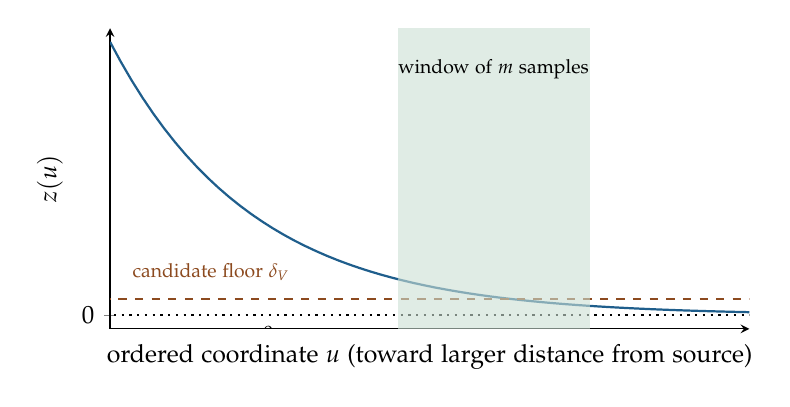
\begin{tikzpicture}
\begin{axis}[width=0.8\textwidth,height=5.4cm,xlabel={ordered coordinate $u$ (toward larger distance from source)},ylabel={$z(u)$},xmin=0,xmax=1,ymin=-0.05,ymax=1.05,xtick=\empty,ytick={0},tick label style={font=\small},label style={font=\small},axis lines=left]
\addplot[domain=0:1,samples=60,thick,accA]{exp(-4.5*x)};
\addplot[dashed,thick,accB]{0.06};
\addplot[dotted,thick,black]{0};
\fill[accC!25,opacity=0.6] (axis cs:0.45,-0.05) rectangle (axis cs:0.75,1.05);
\node[font=\scriptsize] at (axis cs:0.6,0.9) {window of $m$ samples};
\node[font=\scriptsize,anchor=south west,text=accB] at (axis cs:0.02,0.09) {candidate floor $\delta_V$};
\node[font=\scriptsize,anchor=north west] at (axis cs:0.02,-0.005) {vacuum proxy $0$};
\end{axis}
\end{tikzpicture}
\caption{Schematic (not data) of the VREF-I construction. A vacuum-subtracted profile $z(u)$ (blue) decays toward the zero vacuum proxy. A fixed-width window of $m$ ordered samples slides outward; $D_{\rm VREF}(s)$ is the RMS of $z$ over the window. The outcome of interest is whether $D_{\rm VREF}$ keeps decreasing toward the vacuum-compatible region or saturates at a positive floor $\delta_V$ (dashed).}\label{fig:vref}
\end{figure}

\paragraph{Refinement and admissibility.} A primary verdict requires at least three admitted refinement levels on common support; a two-level sequence is only a sensitivity or replication branch. $D_{\rm VREF}$ is not an admissibility test: a profile enters $\AYM$ only if it independently satisfies provenance and representation rules (Yang--Mills-derived provenance, gauge-invariant observable, valid vacuum reference, known coordinate ordering and scale mapping, finite reproducible values, frozen common support, no target-dependent rescue transformation). A small $D_{\rm VREF}$ cannot make an invalid object admissible. STRUC-I may be run on the ordered windows as a secondary \emph{grammar} readout, but it defines neither the vacuum proxy nor the distance.

\subsection{EMT-I: the vacuum-subtracted energy--momentum-tensor representation}\label{ssec:emti}
EMT-I changes the physical representation itself, from connected chromoelectric-field amplitudes to the gradient-flow energy--momentum tensor around a static pair. From the published profile at fixed source separation $R$ it forms the four components $\varepsilon=-T_{44}$, $\sigma_{zz}=-T_{zz}$, $\sigma_{rr}=-T_{rr}$, $\sigma_\theta=-T_{\theta\theta}$ (sign conventions as plotted in the source, preserved alongside the derived values) and the four-component norm. The branch is analyzed on the transverse tail $r\ge R/2$.

\subsection{Floor-versus-zero model competition}\label{ssec:aicc}
Whether a vacuum-directed tail decays to zero or levels off at a positive floor is decided by model competition on the tail. Two families are used, a pure exponential $Ae^{-r/\lambda}$ and a Bessel-$K_0$ form, each in a \emph{zero} version ($k=2$ parameters) and a \emph{positive-floor} version with an additive constant $\delta$ ($k=3$). With Gaussian errors $\mathrm{AICc}=\chi^2+2k+2k(k+1)/(n-k-1)$ for $n$ tail points, and the decision statistic is
\begin{equation}
\Delta\mathrm{AICc}=\mathrm{AICc}_{\rm floor}-\mathrm{AICc}_{\rm zero}.
\end{equation}
Positive values favor the zero floor; the preregistered decisive threshold is $|\Delta\mathrm{AICc}|\ge6$; values below it are \texttt{UNDECIDED}. A \emph{drop-first} sensitivity removes the innermost tail point. This criterion is conservative against a positive-floor claim as well as against a zero-floor claim: an indeterminate result is not evidence for either.

\subsection{Complementary roles}
\Cref{tab:instruments} summarizes what each instrument measures. The key point is that they probe different projections of the same physical object and fail in different ways, which is why agreement across them is informative and why none is allowed to be tuned using another.

\begin{table}[t]
\centering\small
\caption{The instruments, what they measure, and what they cannot say.}\label{tab:instruments}
\begin{tabularx}{\textwidth}{@{}l>{\raggedright\arraybackslash}X>{\raggedright\arraybackslash}X@{}}
\toprule Instrument & Measures & Cannot say\\\midrule
STRUC-I & Order-admissibility of a ladder under perturbation; regime & Distance to the vacuum; spectral content\\
STRUC-PERC-I & Connectivity of the ladder's gap graph & Admissibility; vacuum specificity\\
CORR-I & Compatibility of a correlator with added low-energy weight; massive vs.\ gapless separation at a resolution & Hamiltonian spectrum; refinement stability by itself\\
VREF-I & Vacuum-referenced profile distance along a spatial path & Mass gap; asymptotic limit $D\to0$\\
EMT-I & Independent vacuum-subtracted continuum representation & Same\\
$\Delta$AICc & Zero floor vs.\ positive floor on a tail & Anything beyond the tested tail\\\bottomrule
\end{tabularx}
\end{table}

%==============================================================
\section{The original vacuum non-crossability program}\label{sec:original}

The first project, \texttt{UNNS\_YM\_GAP} (closed 2026-09-30 at stage YM-3B; terminal chamber CORR-I v0.1.2), began from the frozen statement that \emph{gapless Yang--Mills continuation is structurally non-generable under refinement, whereas the massive branch is refinement-stable}. Its stronger form was that the mass gap corresponds to a refinement-stable non-crossability boundary separating the vacuum from every non-vacuum admissible state. We present it in full, because the second project exists only because of how this one ended.

\subsection{Logic of the program}
Let $V$ denote the vacuum and $X$ an admissible non-vacuum structure. The structural hypothesis required $D_{\rm YM}(X,V)\ge\delta_G>0$ surviving refinement. A gapless continuation would instead be a sequence $V\to X_1\to X_2\to\cdots$ with $E(X_n)-E(V)\to0^+$ in which every $X_n$ remains admissible. The intended physical bridge was
\begin{equation}
E(X)-E(V)\;\ge\;F_G\big(D_{\rm YM}(X,V)\big),\qquad F_G(\delta_G)>0,
\end{equation}
a structural-to-Hamiltonian bound that was never reached; the project remained a structural investigation throughout. Four non-negotiable conditions were frozen: (i) gauge-invariant observables; (ii) \emph{adversarial} construction of the gapless continuation rather than inference from the absence of low-energy states; (iii) survival of any obstruction under common refinement; (iv) a strict distinction between a structural diagnostic and a Hamiltonian theorem. Condition (iii) was decisive: a fixed-resolution separation was never sufficient.

\subsection{YM-2A: vacuum-anchored spectral ladders}\label{ssec:ym2a}
The first representation took five glueball-state coordinates available at all eight Athenodorou--Teper ensembles \cite{AT20}---the $A_1^{++}$ ground state (the $0^{++}$ mass-gap state), the $A_1^{++}$ first excitation, the $E^{++}$ and $T_2^{++}$ grounds, and the $A_1^{-+}$ ground---and added an explicit vacuum node, $L^{\rm YM}=(0,x_1,\dots,x_5)$. The vacuum node was essential: without it a common translation of all positive masses leaves adjacent gaps unchanged and is invisible to a gap-based chamber. Four frozen deformation families were then applied along a dyadic sequence $\epsilon=2^{-k}$, $k=0,\dots,10$: \texttt{offset} (translate all positive states downward, vacuum fixed), \texttt{upctrl} (translate upward), \texttt{scale} (multiply all positive states by $\epsilon$), and \texttt{gaponly} (move only the lowest state toward the vacuum).

\paragraph{STRUC-I.} It did not reject the vacuum-compressed branch. Across baselines and the offset family every case remained in Geometric Persistence, with several Stable-Structure/Weak-Persistence changes but no regime transition; the six-node ladder stayed structurally admissible under a factor-1024 compression of the vacuum gap.

\paragraph{STRUC-PERC-I.} It was more sensitive, but the directionality test failed (\cref{tab:ym2a}). Downward vacuum-gap compression often fragmented the pairwise gap graph; so did \emph{upward} translation away from the vacuum; uniform scaling left the normalized connectivity geometry invariant; and gap-only deformation fragmented most strongly. The operative variable was selective displacement of gap coordinates relative to the internal gap distribution under the chamber's IQR normalization, not approach to the vacuum.
\begin{table}[t]
\centering\small
\caption{STRUC-PERC-I outcomes over the $4\times$ deformation families (counts of \texttt{FULL}/\texttt{HARD} fragmentation outcomes, YM-2A).}\label{tab:ym2a}
\begin{tabular}{@{}lcc@{}}\toprule Family & FULL & HARD\\\midrule offset & 19 & 61\\ upctrl & 21 & 59\\ scale & 80 & 0\\ gaponly & 8 & 72\\\bottomrule\end{tabular}
\end{table}
The correct conclusions were that spectral-gap connectivity can collapse while STRUC-I admissibility survives, and that the six-node spectral representation does not establish vacuum-specific non-crossability. This was a successful falsification of a representation/test pair, not of the program.

\subsection{Why a correlator-native chamber}
A short sorted list of extracted masses is already a compressed product of the Euclidean correlation structure. Euclidean two-point functions, $C(t)=\int_0^\infty\rho(E)e^{-Et}dE$ with $\rho\ge0$, retain more direct information about spectral support. The move from STRUC-I/STRUC-PERC-I to CORR-I (\cref{ssec:corri}) was therefore a correction of the representation, not a relaxation of the hypothesis.

\subsection{CORR-I physical-side inputs and the legitimacy of the adversaries}
AT20 does not tabulate the correlator matrix $C_{ij}(t)$; it presents effective-mass plots and the resulting mass estimates. Two controlled physical-side inputs at the finest ensemble ($\beta=6.50$, $38^4$) were therefore built, both explicitly labelled as not being the authors' raw correlators.

\paragraph{Figure-7 proxy.} The $0^{++}$ ground-state effective-mass series of AT20's Fig.~7 was converted into a normalized correlator through $C(0)=1$, $C(n+1)=C(n)\,e^{-aM_{\rm eff}(n+1/2)}$. The reconstruction (11 positive points, no monotonicity violation, four log-convexity violations, no plateau, failed higher-rank Hankel tests) was classified \texttt{SPECTRAL-\allowbreak{}POSITIVITY TENSION}. This was not read as a failure of spectral positivity: AT20 itself discusses the late-time rise of the effective mass as a statistical fluctuation, and exact moment tests are strict enough that a noisy digitized proxy is not expected to pass them. Nevertheless its envelope contraction was strong, $R_{\rm raw}\approx0.00716$.

\paragraph{Published-mass plateau control.} A clean control $C_{\rm massive}(t)=e^{-0.3474\,t}$, $t/a=0,\dots,10$, was built from the published $aM=0.3474(22)$, with the $\pm0.0022$ mass uncertainty kept as a correlated model band and not converted into independent pointwise errors. It passed every baseline test and gave $\alpha_{\max}(1)=0.5$, $\alpha_{\max}(10^{-3})\approx0.0038438$, hence $R_{\rm massive}\approx0.00768765$. The agreement $R_{\rm raw}\approx0.00716$ versus $R_{\rm massive}\approx0.00769$ is the first robustness result: the late-time fluctuation affects the exact positivity tests but does not create the strong near-zero contraction.

\paragraph{Gapless adversaries.} A single gapless control was constructed with $\rho(E)=\theta^{-1}e^{-E/\theta}$, whose spectral support reaches $E=0$, giving $C(t)=1/(1+\theta t)$; the parameter $\theta=e^{0.3474}-1$ was chosen so that the first effective-mass interval matches the massive control, $m_{\rm eff}(0.5)=0.3474$, so that the comparison does not simply contrast different initial scales. This control was positive, monotone, log-convex, Hankel/Hausdorff consistent and without plateau, with $R_{p=1}\approx0.3269$, about $42.5\times$ the massive value. One control is not enough, so the family
\begin{equation}
C_p(t)=(1+\theta_p t)^{-p},\qquad \theta_p=e^{0.3474/p}-1,
\end{equation}
was used, the Laplace transform of the Gamma density $\rho_p(E)=E^{p-1}e^{-E/\theta_p}/(\Gamma(p)\theta_p^{p})$. Every member is exactly gapless (support reaching $E=0$), is matched to $m_{\rm eff}(0.5)=0.3474$, and lives on the same finite interval; the family varies shape while holding the initial mass scale fixed. Three properties make this family the appropriate adversary and not a strawman. (i) Legitimacy: every member is a Laplace transform of a positive measure, so it satisfies exactly the positivity, monotonicity, log-convexity and Hankel/Hausdorff conditions that the baseline layer tests; all five members passed them. (ii) Interpolation: since $\theta_p\sim 0.3474/p$ as $p\to\infty$, $C_p(t)\to e^{-0.3474\,t}$, so the family converges to the massive control, and increasing $p$ makes the adversary progressively \emph{harder}; $p=8$ is the hardest member tested. (iii) Falsifiability: a gapless correlator that looks exponential over a finite window can imitate massive behavior, so no single short correlator can give a binary theorem; what can be asked is whether a measurable separation persists.

\begin{figure}[t]
\centering
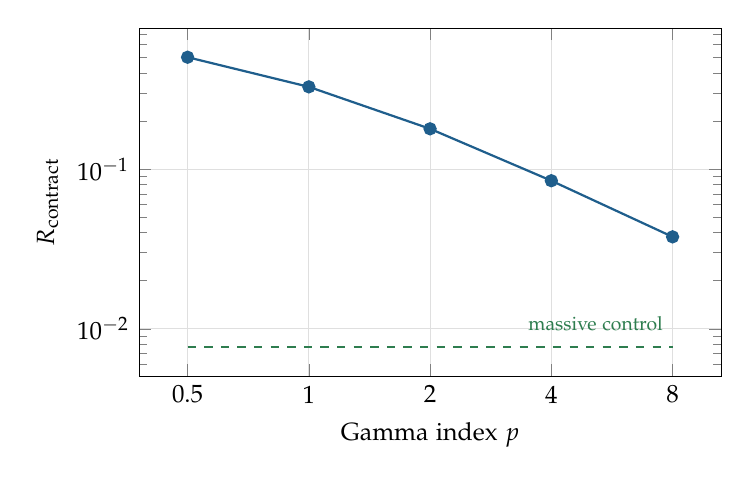
\begin{tikzpicture}
\begin{axis}[width=0.74\textwidth,height=6cm,xmode=log,ymode=log,xlabel={Gamma index $p$},ylabel={$R_{\rm contract}$},xtick={0.5,1,2,4,8},xticklabels={0.5,1,2,4,8},grid=major,grid style={gray!25},tick label style={font=\small},label style={font=\small}]
\addplot[mark=*,thick,accA] coordinates {(0.5,0.500947) (1,0.326916) (2,0.178612) (4,0.084534) (8,0.037668)};
\addplot[dashed,thick,accC] coordinates {(0.5,0.007688)(8,0.007688)};
\node[font=\scriptsize,anchor=south east,text=accC] at (axis cs:8,0.008456) {massive control};
\end{axis}
\end{tikzpicture}
\caption{CORR-I contraction ratio $R_{\rm contract}$ for the matched gapless Gamma family at $\beta=6.50$ (blue) and for the massive plateau control (dashed). The ordering $R_{0.5}>R_1>R_2>R_4>R_8>R_{\rm massive}$ holds; as $p$ grows the adversary approaches the massive response but $R_{p=8}\approx4.90\,R_{\rm massive}$ remains separated.}\label{fig:corr}
\end{figure}

\subsection{YM-2 fixed-resolution result and verdict}
At the finest resolution the contraction ratios were $0.500947$, $0.326916$, $0.178612$, $0.084534$ and $0.037668$ for $p=0.5,1,2,4,8$ against $0.007688$ for the massive control (ratios $65.2\times$, $42.5\times$, $23.2\times$, $11.0\times$ and $4.90\times$), with $\alpha_{\max}^{\rm deep}$ larger for the hardest gapless member by about $1.60$ relative to the massive control at the deepest scan point (\cref{fig:corr}). All gapless members were \texttt{POSITIVE-\allowbreak{}SPECTRAL CONSISTENT}; hence positive spectral consistency alone does not force the massive-side response, and the near-zero contraction is not a trivial consequence of positivity. The stage closed with the provisional verdict \texttt{VACUUM-\allowbreak{}BOUNDARY DIAGNOSTIC ESTABLISHED; REFINEMENT TEST REQUIRED}. The idea thus had genuine empirical motivation: CORR-I did discriminate massive from legitimate gapless controls.

\subsection{YM-3A: model-refinement persistence (Class C)}
The first refinement test used exact mass-anchored exponential controls built from the eight published masses of AT20 \cite{AT20}, with $\beta$-matched Gamma controls at each level. The frozen result was \texttt{MODEL-\allowbreak{}REFINEMENT PERSISTENT}. At all eight levels the massive control stayed on the massive side of the fixed hardest gapless reference ($S_{\rm fixed}>0$) and of every $\beta$-matched control ($S_{\rm match}>0$); the full matched ordering was retained, all forty matched controls were positive-spectral consistent, Hankel/Hausdorff consistent and passed the $\alpha=0$ identity null; and the native-grid window diagnostic did not reverse the separation. The matched margin grew from $S_{\rm match}=0.8067$ at $\beta=5.6924$ to $1.5892$ at $\beta=6.50$ (\cref{fig:ym3a}). The claim boundary was explicit: an exponential built from a published fitted mass carries no measured effective-mass fluctuation, contamination, finite-sample structure or covariance. YM-3A therefore established persistence for a model family, not for measured correlators, and the project prohibited promoting it into a measured-data or continuum claim.

\begin{figure}[t]
\centering
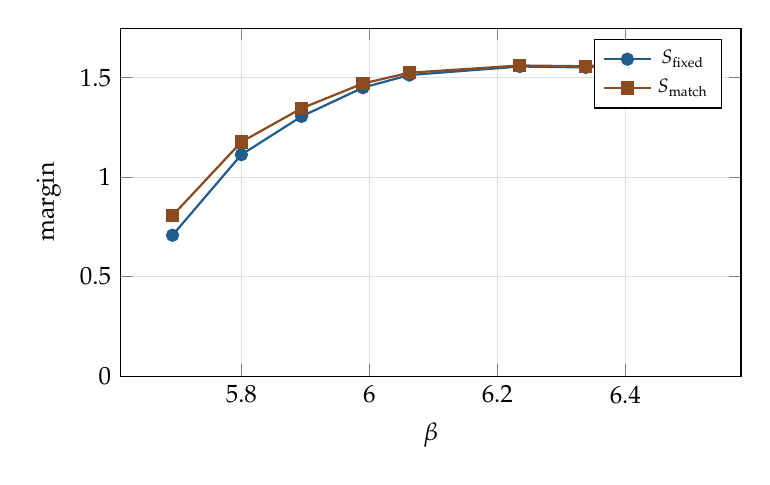
\begin{tikzpicture}
\begin{axis}[width=0.78\textwidth,height=6cm,xlabel={$\beta$},ylabel={margin},ymin=0,grid=major,grid style={gray!25},legend pos=north east,legend style={font=\scriptsize},tick label style={font=\small},label style={font=\small}]
\addplot[mark=*,thick,accA] coordinates {(5.6924,0.70802) (5.8,1.11295) (5.8941,1.30503) (5.99,1.44951) (6.0625,1.51288) (6.235,1.55569) (6.338,1.55128) (6.5,1.58919)};
\addplot[mark=square*,thick,accB] coordinates {(5.6924,0.80671) (5.8,1.17690) (5.8941,1.34576) (5.99,1.47040) (6.0625,1.52449) (6.235,1.56084) (6.338,1.55710) (6.5,1.58919)};
\legend{$S_{\rm fixed}$,$S_{\rm match}$}
\end{axis}
\end{tikzpicture}
\caption{YM-3A (Class C): fixed-reference margin $S_{\rm fixed}$ and $\beta$-matched margin $S_{\rm match}$ against $\beta$ for the eight AT20 ensembles. Both are positive at every level (the two coincide at $\beta=6.50$ by construction).}\label{fig:ym3a}
\end{figure}

\subsection{YM-3B: the measured-data challenge (Class B)}
\paragraph{Source and reconstruction.} The decisive test used four ordered pure-SU(3) ensembles of Sakai and Sasaki \cite{SS23} at $\beta=6.20,\,6.40,\,6.71,\,6.93$: Wilson plaquette action, approximately fixed physical volume $La\approx1.6$\,fm, gauge-invariant spacelike Wilson-loop glueball operators, and a variational analysis with a $6\times6$ correlation matrix. The $A_1^{++}/0^{++}$ ground-state effective-mass trajectories (their Figs.~9--12) were digitized and reconstructed into normalized variational-eigenvalue proxies on a common physical-time grid $u=0.31,0.36,\dots,0.61$ (seven points). All four levels passed input admission. Interpolation (linear primary, PCHIP sensitivity), matched Gamma adversaries, nested ladders and the uncertainty procedure were frozen before the scientific batch.

\paragraph{Central result.} The central margins were $S_B=+0.020350,\,+0.035867,\,-0.003395,\,+0.051851$. At $\beta=6.71$ the matched ordering failed because $R_B>R_{p=8}$: the central trajectory \emph{crossed} the proposed boundary (\cref{tab:ym3b} in \cref{app:data}).

\paragraph{Robustness of the crossing.} The negative sign survived the PCHIP interpolation ($-0.003948$) and all three nested ladder lengths ($S_B^{L5}=-0.007663$, $S_B^{L6}=-0.006666$, $S_B^{L7}=-0.003395$; \cref{fig:ladder}). It therefore could not be dismissed as an artifact of the interpolation rule or of the choice of five, six or seven common-grid points.

\paragraph{Why it is not a falsification.} The preregistered 2000-draw pointwise-no-covariance ensemble at $\beta=6.71$ gave a $95\%$ interval $[-0.027454,\,+0.019320]$, median $-0.003285$, with $60.65\%$ of draws negative and $39.35\%$ positive, while the other three levels were sign-stable (\cref{fig:SB}). Under the frozen rule digitization/statistical uncertainty dominates the sign of the only central crossing and the verdict is \texttt{DATA-\allowbreak{}INDETERMINATE}. A further limitation: all four reconstructed baselines were classified \texttt{SPECTRAL-\allowbreak{}POSITIVITY TENSION} under the strict moment checks, consistent with their provenance as digitized trajectories rather than covariance-preserving correlators, and the $\beta=6.93$ reconstruction did not satisfy the plateau detector even though its margin remained positive. The crossing is not erased; it is not promoted beyond the precision of the source.

\begin{figure}[t]
\centering
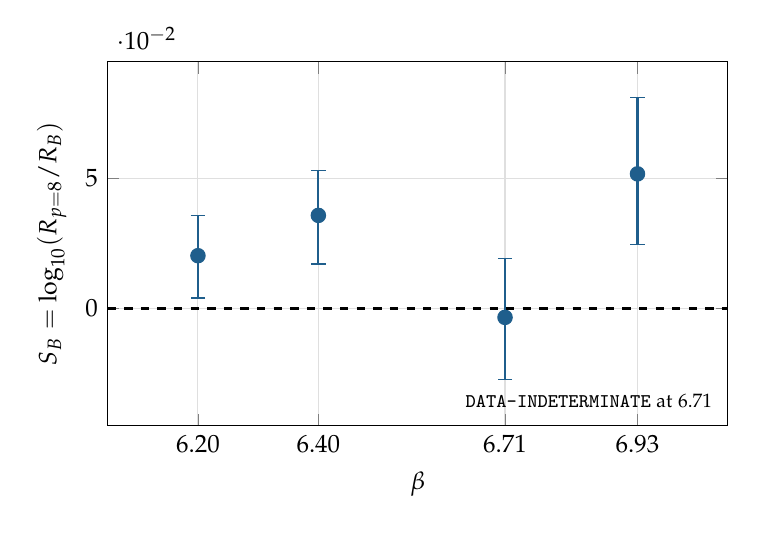
\begin{tikzpicture}
\begin{axis}[width=0.78\textwidth,height=6.2cm,xlabel={$\beta$},ylabel={$S_B=\log_{10}(R_{p=8}/R_B)$},xmin=6.05,xmax=7.08,ymin=-0.045,ymax=0.095,xtick={6.2,6.4,6.71,6.93},xticklabels={6.20,6.40,6.71,6.93},grid=major,grid style={gray!25},tick label style={font=\small},label style={font=\small}]
\addplot[dashed,thick,black] coordinates {(6.05,0)(7.08,0)};
\addplot[only marks,mark=*,mark size=2.6pt,accA,error bars/.cd,y dir=both,y explicit,error bar style={thick}] table[row sep=\\,x index=0,y index=1,y error plus index=2,y error minus index=3] {
6.2 0.020350 0.015308 0.016297\\
6.4 0.035867 0.017227 0.018700\\
6.71 -0.003395 0.022715 0.024059\\
6.93 0.051851 0.029343 0.027126\\
};
\node[font=\scriptsize,anchor=south east] at (axis cs:7.07,-0.042) {\texttt{DATA-\allowbreak{}INDETERMINATE} at 6.71};
\end{axis}
\end{tikzpicture}
\caption{Class B margin $S_B=\log_{10}(R_{p=8}/R_B)$ at the four Sakai--Sasaki ensembles \cite{SS23}. Dots: central values; bars: preregistered 2000-draw 95\% intervals (2.5\%--97.5\% quantiles); dashed line: the proposed boundary $S_B=0$. Only $\beta=6.71$ is sign-unstable, and there the interval straddles zero.}\label{fig:SB}
\end{figure}
\begin{figure}[t]
\centering
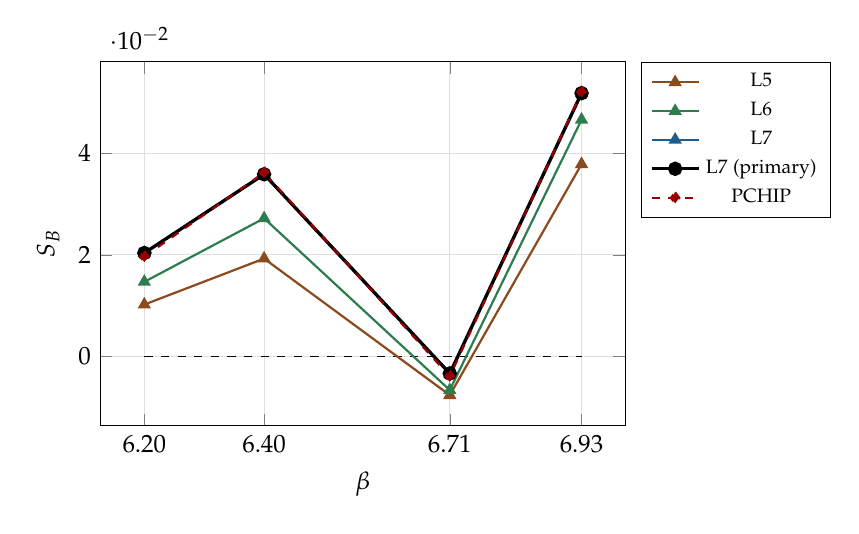
\begin{tikzpicture}
\begin{axis}[width=0.68\textwidth,height=6.2cm,xlabel={$\beta$},ylabel={$S_B$},xtick={6.2,6.4,6.71,6.93},xticklabels={6.20,6.40,6.71,6.93},grid=major,grid style={gray!25},legend pos=outer north east,legend style={font=\scriptsize},tick label style={font=\small},label style={font=\small}]
\addplot[dashed,black] coordinates {(6.2,0)(6.93,0)};
\addplot[mark=triangle*,thick,accB] coordinates {(6.2,0.010186) (6.4,0.019249) (6.71,-0.007663) (6.93,0.037860)};
\addplot[mark=triangle*,thick,accC] coordinates {(6.2,0.014667) (6.4,0.027185) (6.71,-0.006666) (6.93,0.046615)};
\addplot[mark=triangle*,thick,accA] coordinates {(6.2,0.020350) (6.4,0.035867) (6.71,-0.003395) (6.93,0.051851)};
\addplot[mark=*,very thick,black] coordinates {(6.2,0.020350) (6.4,0.035867) (6.71,-0.003395) (6.93,0.051851)};
\addplot[mark=diamond*,thick,red!60!black,dashed] coordinates {(6.2,0.019648) (6.4,0.036198) (6.71,-0.003948) (6.93,0.052060)};
\legend{,L5,L6,L7,L7 (primary),PCHIP}
\end{axis}
\end{tikzpicture}
\caption{Sensitivity of the central margin to the nested common-grid ladder length (L5, L6, L7 points) and to PCHIP interpolation. At $\beta=6.71$ the sign is negative in every variant.}\label{fig:ladder}
\end{figure}

\subsection{Closure and what it taught}
The central hypothesis was recorded as \texttt{NOT ESTABLISHED}. YM-4 (a bridge theorem under the original premise) was not entered, and further tests (Liang et al.\ replication, extension to Chen et al., additional source search, CORR-I redesign to restore the separation) were cancelled. The record does \emph{not} call the picture refuted, does not claim that no structural boundary exists, and neither proves nor disproves the physical mass gap. It left five lessons that carry directly into the second project: connectivity is not admissibility; representation depth matters, since a short sorted mass ladder erases distinctions that the Euclidean correlator retains; positive spectral consistency does not determine the near-zero response; a finite-window gapless spectrum can approach massive-looking behavior continuously; and model-level persistence does not imply measured-data persistence, so evidence classes must stay separated.

It also left one consequence at the level of \uns{} ontology. The picture implicit in the original program was
\[
\text{admissible structure}\ \Big|\ \text{forbidden region}\ \Big|\ V ,
\]
and the experiments did not support that geometry. The more faithful reading is
\[
\text{admissible structure}\longrightarrow\text{increasingly vacuum-like structure}\longrightarrow V
\]
inside a common structural domain: the vacuum behaves as an internal structural regime or locus of the substrate and not as an exterior beyond it. This is a structural interpretation, not a theorem about quantum field theory, and it is the starting point of the second project.

%==============================================================
\section{From non-crossability to structural accessibility}\label{sec:pivot}

The pivot is conceptual. A mass gap separates \emph{eigenvalues}; a structural neighborhood describes \emph{configurations or observables}. These live in different spaces with no a priori common topology, so a spectral gap need not induce a structural wall. The second project, \texttt{UNNS\_VACUUM\_CONTINUITY}, froze the corresponding ontology in its Stage~1: the vacuum is an \emph{internal closure object} of the admissible domain,
\begin{equation}
V\in\overline{\AYM\setminus\{V\}},\qquad\text{primary hypothesis}\quad \inf_{X\in\AYM\setminus\{V\}}\Dstruct(X,V)=0,
\end{equation}
against the isolation alternative: $\exists\,\delta_V>0$ with $\Dstruct(X,V)\ge\delta_V$ for every sufficiently refined admissible non-vacuum structure in the tested representation class. Stage~1 deliberately did \emph{not} adopt the language ``basin'', ``attractor'' or ``fixed point'', which would require further evidence. Its physical shorthand, frozen as interpretive and not theorem-level, is that the mass gap separates eigenvalues, not necessarily structural neighborhoods.

\paragraph{Frozen requirements.} Within VREF-I, evidence for structural vacuum continuity required all of: at least three admitted refinement levels; a documented independent vacuum baseline or explicit connected subtraction; common physical support; fixed-width ordered windows; decreasing or vacuum-compatible $D_{\rm VREF}$ toward the independently identified asymptotic region; no refinement-stable positive lower bound resolved above uncertainty; persistence under the preregistered metric and interpolation sensitivities; no loss of admissibility; and no dependence on CORR-I. A finite dataset can support structural continuity \emph{over its tested domain}; it cannot by itself prove the infinite-resolution statement $\Dstruct\to0$.

\paragraph{Frozen falsification condition.} Within the tested representation class, the continuity hypothesis is contradicted if sufficiently refined admitted data establish a stable nonzero exclusion scale $D_{\rm VREF}\ge\delta_V>0$ through the full vacuum-directed region, surviving common refinement, uncertainty propagation, the frozen secondary metric and independent profile construction. If the vacuum reference is inadequate, the common grid fails, or uncertainties dominate the putative bound, the verdict is \emph{indeterminate}, not isolation-supported. Seven specific failure modes F1--F7 were enumerated in advance (\cref{tab:F}).

\paragraph{Separation from the spectral side.} Three quantities are kept distinct: $D_{\rm VREF}$, the structural profile distance; $\Delta_{\rm spec}$, a measured or reconstructed positive spectral scale; and $\Delta_{\rm YM}$, the physical continuum Yang--Mills mass gap. Stage~2 addresses the first; Stage~3 tests whether the first coexists with the second in the same theory.

%==============================================================
\section{A structural--spectral separation theorem}\label{sec:theorem}

\Cref{sec:pivot} suggests that the original program was implicitly assuming a bridge from spectral energy to structural distance. This section proves what such a bridge would give, and what its absence allows.

\subsection{Setting}
\begin{definition}[Structural--spectral system]
A \emph{structural--spectral system} $(\mathcal S,d,V,\Pset,\varepsilon)$ consists of a metric space $(\mathcal S,d)$ of structural states; a vacuum $V\in\mathcal S$; a set $\Pset\subseteq\mathcal S\setminus\{V\}$ of \emph{physical non-vacuum excitations}; and an \emph{excitation-energy functional} $\varepsilon:\mathcal S\to[0,\infty)$ with $\varepsilon(V)=0$. It is \emph{gapped} with gap $\Delta>0$ if
\begin{equation}\label{eq:gap}
\varepsilon(X)\ge\Delta\qquad\text{for all }X\in\Pset .
\end{equation}
It has a \emph{structural exclusion radius} $\delta>0$ if $d(X,V)\ge\delta$ for all $X\in\Pset$, i.e.\ $B_\delta(V)\cap\Pset=\varnothing$ for the open ball $B_\delta(V)=\{X:d(X,V)<\delta\}$. It is \emph{structurally accessible} if there is a sequence $X_n\in\Pset$ with $d(X_n,V)\to0$.
\end{definition}
Thus $\Hiso$ asserts an exclusion radius, and $\Hacc^{\rm lim}$ asserts structural accessibility, both under a gap. The set $\mathcal S$ may contain non-physical states; this matters in \cref{rem:nonnec}.

\begin{theorem}[Structural--spectral separation]\label{thm:sep}
Let $(\mathcal S,d,V,\Pset,\varepsilon)$ be gapped with gap $\Delta>0$.
\begin{enumerate}[label=(\alph*)]
\item \textbf{A gap alone does not imply a structural gap.} There exist gapped systems with $\inf_{X\in\Pset}d(X,V)=0$; so $\Delta>0$ does not imply an exclusion radius.
\item \textbf{Continuity is a sufficient bridge.} If $\varepsilon$ is continuous at $V$, then there is $\delta>0$ with $B_\delta(V)\cap\Pset=\varnothing$.
\item \textbf{Accessibility forces discontinuity.} If there are $X_n\in\Pset$ with $d(X_n,V)\to0$, then $\varepsilon$ is discontinuous at $V$; its oscillation there satisfies $\limsup_{X\to V}|\varepsilon(X)-\varepsilon(V)|\ge\Delta$.
\item \textbf{Factorization obstruction.} Let $(\mathcal Y,\tau)$ be a topological space (a ``spectral-state space''), $\Pi:\mathcal S\to\mathcal Y$ and $\mathcal E:\mathcal Y\to[0,\infty)$ with $\varepsilon=\mathcal E\circ\Pi$, and put $\Omega=\Pi(V)$, so $\mathcal E(\Omega)=0$. If $\Pset$ contains a sequence $X_n\to V$ in $(\mathcal S,d)$, then at least one of the following fails: $\Pi$ is continuous at $V$ (into $\tau$); $\mathcal E$ is continuous at $\Omega$ (in $\tau$).
\item \textbf{Quantitative form.} Suppose there are $r>0$, $C>0$, $\alpha>0$ with $\varepsilon(X)\le C\,d(X,V)^\alpha$ whenever $d(X,V)<r$. Then every $X\in\Pset$ satisfies
\begin{equation}\label{eq:holder}
d(X,V)\;\ge\;\delta_{\rm struct}:=\min\!\Big\{\,r,\ \Big(\tfrac{\Delta}{C}\Big)^{1/\alpha}\Big\}.
\end{equation}
If the Hölder bound holds globally ($r=\infty$), $\delta_{\rm struct}=(\Delta/C)^{1/\alpha}$.
\end{enumerate}
\end{theorem}

\begin{proof}
\textbf{(a)} Take $\mathcal S=\{0\}\cup\{1/n:n\in\mathbb N\}\subset\mathbb R$ with the Euclidean metric, $V=0$, $\Pset=\{1/n:n\in\mathbb N\}$, and $\varepsilon(0)=0$, $\varepsilon(1/n)=1$ for all $n$. Then $\varepsilon\ge\Delta:=1$ on $\Pset$, so the system is gapped; yet $d(1/n,V)=1/n\to0$, so $\inf_{X\in\Pset}d(X,V)=0$ and no exclusion radius exists.

\textbf{(b)} Put $\eta=\Delta/2$. By continuity at $V$ there is $\delta>0$ with $d(X,V)<\delta\Rightarrow|\varepsilon(X)-\varepsilon(V)|<\Delta/2$, i.e.\ $\varepsilon(X)<\Delta/2$ because $\varepsilon(V)=0$. If some $X\in\Pset$ had $d(X,V)<\delta$, then $\Delta\le\varepsilon(X)<\Delta/2$, impossible since $\Delta>0$. Hence $B_\delta(V)\cap\Pset=\varnothing$.

\textbf{(c)} Suppose $\varepsilon$ were continuous at $V$. Then $X_n\to V$ would give $\varepsilon(X_n)\to\varepsilon(V)=0$, contradicting $\varepsilon(X_n)\ge\Delta>0$. For the oscillation: $|\varepsilon(X_n)-\varepsilon(V)|=\varepsilon(X_n)\ge\Delta$ along a sequence converging to $V$.

\textbf{(d)} Suppose, for contradiction, that $\Pi$ is continuous at $V$ and $\mathcal E$ is continuous at $\Omega=\Pi(V)$. A composition of maps continuous at the relevant points is continuous at $V$, so $\varepsilon=\mathcal E\circ\Pi$ is continuous at $V$ in $(\mathcal S,d)$, contradicting (c). (Only the definition of continuity at a point is used; no countability assumption on $\tau$ is needed.)

\textbf{(e)} Let $X\in\Pset$ and suppose $d(X,V)<\delta_{\rm struct}$. Then $d(X,V)<r$, so $\varepsilon(X)\le C\,d(X,V)^\alpha$; and $d(X,V)<(\Delta/C)^{1/\alpha}$ gives $C\,d(X,V)^\alpha<\Delta$. Hence $\varepsilon(X)<\Delta$, contradicting \eqref{eq:gap}. So $d(X,V)\ge\delta_{\rm struct}$.
\end{proof}

\begin{remark}[Continuity is sufficient, not necessary]\label{rem:nonnec}
Part (b) does not say that exclusion \emph{requires} continuity of $\varepsilon$. Take $\mathcal S=\mathbb R$, $V=0$, $\Pset=[1,2]$, $\varepsilon=1$ on $\Pset$, $\varepsilon=5$ on $(0,\tfrac12)$ and $\varepsilon=0$ elsewhere. The system is gapped ($\Delta=1$) and has exclusion radius $1$, yet $\varepsilon$ is discontinuous at $V$, because non-physical states in $(0,\frac12)$ carry energy. Continuity at $V$ therefore provides a \emph{sufficient} bridge from a gap to exclusion; the accurate summary is: a positive gap does not by itself imply a structural exclusion neighborhood; continuity of $\varepsilon$ at $V$ supplies such an implication; and accessibility under a persistent gap rules the continuity out.
\end{remark}

\begin{remark}[Sharpness of \eqref{eq:holder}]
On $\mathcal S=[0,\infty)$, $V=0$, $\varepsilon(x)=Cx^\alpha$ and $\Pset=\{x\ge(\Delta/C)^{1/\alpha}\}$ the system is gapped with gap $\Delta$ and its exclusion radius equals $(\Delta/C)^{1/\alpha}$ exactly, so the constant cannot be improved in general.
\end{remark}

\begin{corollary}[Topological reading]\label{cor:top}
Let $d_\varepsilon(X,Y)=|\varepsilon(X)-\varepsilon(Y)|$ be the energy pseudometric. If the system is gapped and structurally accessible, the identity map $(\mathcal S,d)\to(\mathcal S,d_\varepsilon)$ is discontinuous at $V$: the set $\{\varepsilon<\Delta/2\}$, a $d_\varepsilon$-neighborhood of $V$, is not a $d$-neighborhood of $V$. The structural topology therefore fails to be finer than the energy topology at the vacuum.
\end{corollary}
\begin{proof}
$\{\varepsilon<\Delta/2\}$ contains $V$ and is open for $d_\varepsilon$ but contains no point of $\Pset$, whereas every $d$-ball about $V$ contains some $X_n\in\Pset$ for large $n$.
\end{proof}

\subsection{Illustrations}
\begin{example}[Amplitude-vanishing gapped correlators]\label{ex:corr}
Let $\mathcal S_\Delta$ consist of the zero correlator $V\equiv0$ together with all $C_\nu(t)=\int_{[\Delta,\infty)}e^{-Et}\,d\nu(E)$, $t\ge0$, $\nu$ a nonzero finite positive measure, with $d(C,C')=\sup_{t\ge0}|C(t)-C'(t)|$. Set $\varepsilon(C_\nu)=\inf\operatorname{supp}\nu\ge\Delta$, $\varepsilon(V)=0$, $\Pset=\mathcal S_\Delta\setminus\{V\}$. Since $C_\nu$ is decreasing, $d(C_\nu,V)=C_\nu(0)=\nu([\Delta,\infty))$. For $\nu_n=\tfrac1n\delta_\Delta$ we get $d(C_{\nu_n},V)=1/n\to0$ while $\varepsilon(C_{\nu_n})=\Delta$ for all $n$. This system is gapped and structurally accessible, and $\varepsilon$ is discontinuous at $V$ by \cref{thm:sep}(c).
\end{example}
\begin{example}[A Hilbert-space instance]\label{ex:hilbert}
Let $H$ be a self-adjoint operator on a Hilbert space $\mathcal H$ with a simple eigenvalue $E_0=0$ (eigenvector $\Omega$) and $\sigma(H)\setminus\{0\}\subset[\Delta,\infty)$. For a unit vector $\psi$ write $\psi_\perp=\psi-\langle\Omega,\psi\rangle\Omega$ and let $\mu_\perp$ be the spectral measure of $H$ in $\psi_\perp$; define $\varepsilon(\psi)=\inf\operatorname{supp}\mu_\perp$ if $\psi_\perp\ne0$ and $\varepsilon(\psi)=0$ otherwise, and let $\Pset$ be the set of unit vectors with $\psi_\perp\ne0$. Then $\varepsilon\ge\Delta$ on $\Pset$. For $\psi_\theta=\cos\theta\,\Omega+\sin\theta\,\varphi$ with $\varphi\perp\Omega$, $\|\varphi\|=1$, in the spectral subspace of $[\Delta,\infty)$, we have $\psi_\theta\in\Pset$, $\|\psi_\theta-\Omega\|\to0$ as $\theta\to0$, and $\varepsilon(\psi_\theta)\ge\Delta$ for every $\theta$; moreover $|\langle\psi_\theta,O\psi_\theta\rangle-\langle\Omega,O\Omega\rangle|\to0$ for every bounded operator $O$. Here accessibility holds in the norm and observable topologies while the support-edge functional $\varepsilon$ is norm-discontinuous at the vacuum. This is a generic illustration of the theorem and says nothing about how \uns{} structure maps into a Yang--Mills Hilbert space.
\end{example}
The first example is a toy, not a Yang--Mills statement. It shows that the answer to ``does a gap imply a wall?'' depends on the structural metric: an amplitude-sensitive distance sees spectral weight tending to zero as the vacuum is approached, whereas a shape-normalized distance of the kind a ratio-based diagnostic such as $R_{\rm contract}$ uses would not assign the vacuum a point in the space at all. The second shows that the same phenomenon occurs in the Hilbert-space topologies in which one would hope to formulate the Yang--Mills problem. Choosing the topology on $\SUNNS$ is part of the open problem.

\subsection{Status: what is and is not claimed}
\begin{remark}[Do not oversell]\label{rem:oversell}
\Cref{thm:sep} is essentially a statement about continuity at a point; it is mathematically valid and complete as stated but elementary, and we do not present it as a major theorem. Its value is diagnostic: it makes the missing premise of the original program explicit. $\Hiso$ was effectively the implication $\Delta>0\Rightarrow\Dstruct(X,V)\ge\delta>0$; by (a) that implication is not automatic, and by (b) and (e) it holds under an additional bridge condition such as \eqref{eq:holder}.
\end{remark}
\begin{remark}[The premise is not empirically instantiated]\label{rem:premise}
Parts (c)--(d) assume a sequence of \emph{physical excitations} $X_n\to V$ in a representation-independent structural metric. The experiments do not establish this. The Stage-2 structural states are spatial profile windows and ladders of vacuum-subtracted observables (\cref{sec:stage2}), not excitation sequences carrying a prescribed energy functional, and no representation-independent $\Dstruct$ is constructed. The experiments support accessibility empirically ($\Hacc^{\rm emp}$); they do not discharge the premise of the theorem ($\Hacc^{\rm lim}$). The coexistence claim of \cref{sec:bridge} therefore lives inside the frozen evidence architecture and is not an application of \cref{thm:sep} to Yang--Mills.
\end{remark}
\begin{remark}[On the space $\mathcal Y$]
In (d) the space $\mathcal Y$ is deliberately abstract: ``energy'' is not a scalar function naturally defined on arbitrary Hilbert-space vectors, so at this stage we take $\mathcal Y$ to be a spectral-state/data space on which a functional $\mathcal E$ is specified, and reserve an actual Hilbert-space realization (such as the support-edge functional of \cref{ex:hilbert}) for the future Yang--Mills construction. We write $\Yspec$ for this space when it is instantiated for \uns{}.
\end{remark}

%==============================================================
\section{Stage 2: testing structural vacuum accessibility}\label{sec:stage2}

Stage~2 of \texttt{UNNS\_VACUUM\_CONTINUITY} is the main empirical body. It asks whether any admitted representation yields a refinement-stable positive structural exclusion floor around the vacuum. Success was not defined as one negative diagnostic value. The test required a combination of common refinement, vacuum-directed physical profiles, asymptotic zero-floor versus positive-floor competition, uncertainty control, independent structural chambers, smoothing sensitivity, an independent operator/representation change, geometry sensitivity, and preservation of negative and indeterminate results without retuning. The important point is not that every branch was positive; it is that the negative and limited branches repeatedly failed to produce the universal positive floor that non-crossability demands, and that those that could not decide were preserved as such.

Each branch below is described with the same structure: \emph{data} $\to$ \emph{construction} $\to$ \emph{decision rule} $\to$ \emph{result} $\to$ \emph{sensitivity} $\to$ \emph{what the verdict permits and forbids}. The six branches and their frozen verdicts are summarized in \cref{tab:stage2}.

\begin{table}[t]
\centering\small
\caption{Stage 2 branches at a glance.}\label{tab:stage2}
\begin{tabularx}{\textwidth}{@{}l>{\raggedright\arraybackslash}p{3.1cm}>{\raggedright\arraybackslash}p{3.5cm}>{\raggedright\arraybackslash}X@{}}
\toprule Branch & Data & Instrument & Frozen verdict\\\midrule
7.1 & Baker et al.\ \cite{Baker22}, 3 resolutions & VREF-I/A calibration & \texttt{CALIBRATION-\allowbreak{}SENSITIVE}\\
7.2 & Cea et al.\ \cite{Cea17}, 2 refinements & VREF-I/B & \texttt{REFINEMENT-\allowbreak{}INDETERMINATE}\\
7.3 & Cea et al., 5 ladders & STRUC-I, STRUC-PERC-I & \texttt{ARCHITECTURE-\allowbreak{}PRESERVED}\\
7.4 & Battelli--Bonati \cite{Battelli19}, 3 ladders & STRUC-I, STRUC-PERC-I & \texttt{UNSMOOTHED-\allowbreak{}ARCHITECTURE-\allowbreak{}CONSISTENT}\\
7.5 & Yanagihara et al.\ \cite{Yanagihara19}, $R=0.69$\,fm & EMT-I & \texttt{EMT-\allowbreak{}UNCERTAINTY-\allowbreak{}LIMITED}\\
7.6 & Same, $R=0.46,\,0.92$\,fm & EMT-I & \texttt{GEOMETRY-\allowbreak{}ROBUST-\allowbreak{}NO-\allowbreak{}FLOOR}\\\bottomrule
\end{tabularx}
\end{table}

\subsection{Baker 2022: VREF-I/A calibration}\label{ssec:baker}
\paragraph{Data and construction.} Three pure-SU(3) resolutions of the flux-tube data of Baker et al.\ \cite{Baker22}: R1 ($\beta=6.240$, 33 rows), R2 ($\beta=6.544$, 25 rows) and R3 ($\beta=6.769$, 33 rows), each mirror-symmetric in transverse distance, with native supports $[-1.022,1.022]$\,fm for R1 and $[-0.511,0.511]$\,fm for R2 and R3. All three files passed the frozen SHA-256, finite-value, three-column, non-negative-error, mirror-symmetry, ordering and common-support checks. The frozen geometry: reference length $d=0.511$\,fm, $u=x_t/d$, common grid $u=0,0.125,\dots,1$, window width $W=0.5$, window size $m=5$, linear interpolation as primary and PCHIP as sensitivity, extrapolation prohibited.
\paragraph{Decision rule.} For each window the RMS profile discrepancies $R_{12},R_{23},R_{13}$ between refinement levels are computed, and the contraction ratio $C=R_{23}/R_{12}$ asks whether the medium--fine discrepancy is smaller than the coarse--medium one. \texttt{CALIBRATION-\allowbreak{}SENSITIVE} is assigned if the PCHIP sensitivity changes at least one qualitative property: a profile sign, the direction signature of the $D_{\rm RMS}$ path, the class of $C$ relative to $1$, or the ordering of $R_{12},R_{23},R_{13}$ in any window; otherwise, after integrity checks, \texttt{CALIBRATION-\allowbreak{}VALID}.
\paragraph{Result.} Only window~3 ($u=0.375$) changes qualitative class: $C=0.987$ ($<1$) with linear interpolation and $C=1.036$ ($>1$) with PCHIP, with the refinement-distance ordering changing as well (\cref{fig:baker}). The inner windows 0--2 have $C<1$ under both interpolations (medium--fine discrepancy smaller than coarse--medium, interpolation-robustly), and the outermost window 4 has $C>1$ under both ($1.485$ linear, $1.529$ PCHIP), so the loss of refinement contraction at the largest transverse distance is not produced by the interpolator. The fixed-window distance $D_{\rm VREF}$ decreases monotonically outward at every level under both interpolations (R1: $1.821\to0.614$, R2: $1.862\to0.653$, R3: $1.880\to0.684$, i.e.\ $-66\%$, $-65\%$, $-64\%$), but terminal values remain substantially positive.
\paragraph{Sensitivity diagnosis.} The sensitivity is localized, not global, and it is a grid-commensurability effect in R2: the common grid spacing $0.0639$\,fm is aligned with every R1 native step and every second R3 step ($a\approx0.0639,0.0426,0.0320$\,fm for R1--R3), but many common-grid points fall midway between R2 native points. The maximum dimensionless interpolation difference is $0.0178$ for R2 against $1.1\times10^{-4}$ for R1 and $7.6\times10^{-5}$ for R3; for R2 it is about $1.18$ times the published pointwise error scale. The window~3 flip occurs because $C$ lies almost exactly at unity. A descriptive leave-one-out diagnostic shows that interpolation curvature can exceed the pointwise error on the coarser profiles (median $|r|/\epsilon$ of $3.04,2.17,0.50$ for R1--R3). A post hoc native-aligned diagnostic at $u\in\{0,0.25,0.5,0.75,1\}$ gives $C\approx0.927$; it is diagnostic only and cannot alter the frozen outcome.
\paragraph{What the verdict permits and forbids.} \texttt{CALIBRATION-\allowbreak{}SENSITIVE} forbids reading the branch as \texttt{CONTINUITY-\allowbreak{}SUPPORTED} or \texttt{ISOLATION-\allowbreak{}SUPPORTED}; the common support ends at $0.511$\,fm, so the branch does not test the asymptotic vacuum-compatible region. Its contribution is methodological: a structural-vacuum conclusion cannot rest on an interpolation-sensitive common-refinement construction. Three design lessons were frozen for the next branch: prefer natively common coordinates, make interpolation explicit in the uncertainty if it is unavoidable, and require access farther into the vacuum-compatible tail.

\begin{figure}[t]
\centering
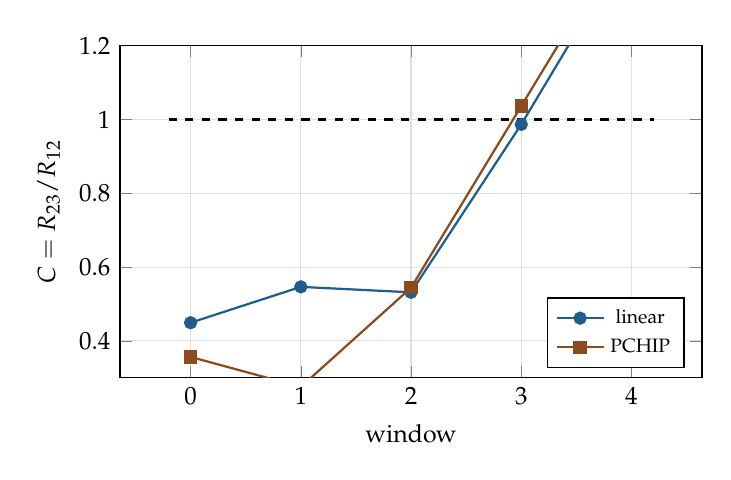
\begin{tikzpicture}
\begin{axis}[width=0.74\textwidth,height=5.8cm,xlabel={window},ylabel={$C=R_{23}/R_{12}$},xtick={0,1,2,3,4},ymin=0.3,ymax=1.2,grid=major,grid style={gray!25},legend pos=south east,legend style={font=\scriptsize},tick label style={font=\small},label style={font=\small}]
\addplot[dashed,thick,black,forget plot] coordinates {(-0.2,1)(4.2,1)};
\addplot[mark=*,thick,accA] coordinates {(0,0.4493) (1,0.5464) (2,0.5317) (3,0.9867) (4,1.4851)};
\addplot[mark=square*,thick,accB] coordinates {(0,0.3566) (1,0.2754) (2,0.5441) (3,1.0364) (4,1.5287)};
\legend{linear,PCHIP}
\end{axis}
\end{tikzpicture}
\caption{VREF-I/A calibration: contraction ratio $C=R_{23}/R_{12}$ by window, linear versus PCHIP interpolation. The classification relative to $C=1$ (dashed) flips only in window~3, where both values lie within $4\%$ of unity.}\label{fig:baker}
\end{figure}

\subsection{Cea et al.\ 2017: VREF-I/B}\label{ssec:cea}
\paragraph{Data and construction.} The connected chromoelectric-field profile of Cea et al.\ \cite{Cea17} supplies two physical refinements (R1, R2) with a deep vacuum-directed tail and an explicit zero-field vacuum reference. The extraction is deterministic (22 rows; 9 common-grid points; common support $0$ to $0.762$\,fm; primary tail cut $x\ge0.380$\,fm giving 5 tail points) and was hashed before analysis.
\paragraph{Decision rules.} Three questions: is the path vacuum-directed (linear and PCHIP); does the zero-floor or positive-floor model win on the tail (\cref{ssec:aicc}); and do the two refinements agree on the absolute amplitude (the frozen refinement-consistency rule).
\paragraph{Result.} The path is \texttt{VACUUM-\allowbreak{}DIRECTED} under both linear and PCHIP interpolation, with no interpolation sensitivity. The floor-model comparison gives $\Delta\mathrm{AICc}=5.238$ for both the exponential and $K_0$ families on the primary tail (\texttt{UNDECIDED}, just below $6$), and $7.200$ for both under the drop-first sensitivity (\texttt{ZERO}, crossing the decisive threshold in favor of the zero floor) (\cref{fig:aicc}). The refinement check fails: $\chi^2_{\rm ref}/N_{\rm tail}=46.05$ with a \emph{structured} mismatch, the second refinement's tail amplitude exceeding the first's by factors $1.07$--$1.18$ over $x=0.38$--$0.76$\,fm (\cref{fig:cea}).
\paragraph{What the verdict permits and forbids.} The zero-floor model is preferred qualitatively and, under drop-first, decisively; but the full preregistered branch cannot be promoted, because the amplitude mismatch means the two refinements do not agree on an absolute vacuum-distance calibration. \texttt{REFINEMENT-\allowbreak{}INDETERMINATE} was preserved unchanged. It is not evidence for isolation; it is evidence that the primary CEA observable does not yet provide a refinement-stable absolute calibration. The branch reports a vacuum-directed structural path with no detected positive floor.

\begin{figure}[t]
\centering
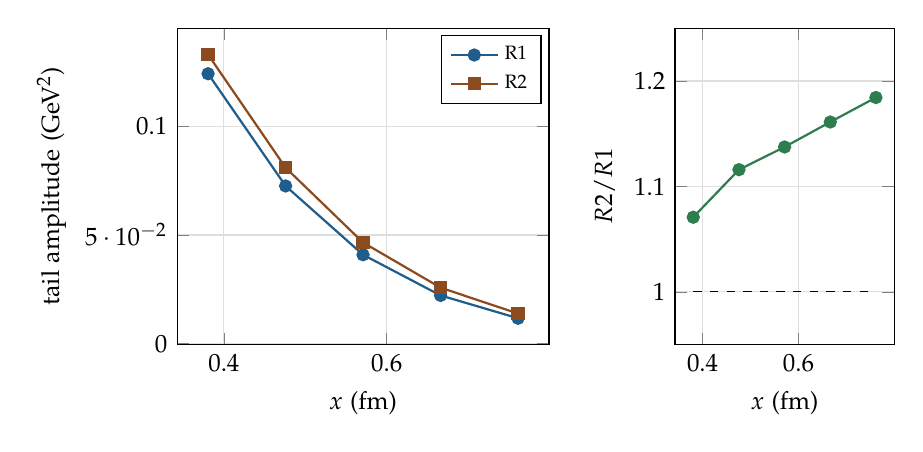
\begin{tikzpicture}
\begin{axis}[name=L,width=0.52\textwidth,height=5.6cm,xlabel={$x$ (fm)},ylabel={tail amplitude (GeV$^2$)},grid=major,grid style={gray!25},legend style={font=\scriptsize},tick label style={font=\small},label style={font=\small}]
\addplot[mark=*,thick,accA] coordinates {(0.3806,0.12421) (0.4758,0.07257) (0.5709,0.04093) (0.6661,0.02221) (0.7612,0.01171)};
\addplot[mark=square*,thick,accB] coordinates {(0.3806,0.13301) (0.4758,0.08098) (0.5709,0.04655) (0.6661,0.02579) (0.7612,0.01387)};
\legend{R1,R2}
\end{axis}
\begin{axis}[at={(L.east)},xshift=1.6cm,anchor=west,width=0.36\textwidth,height=5.6cm,xlabel={$x$ (fm)},ylabel={$R2/R1$},ymin=0.95,ymax=1.25,grid=major,grid style={gray!25},tick label style={font=\small},label style={font=\small}]
\addplot[dashed,black] coordinates {(0.381,1)(0.761,1)};
\addplot[mark=*,thick,accC] coordinates {(0.3806,1.0708) (0.4758,1.1159) (0.5709,1.1374) (0.6661,1.1611) (0.7612,1.1843)};
\end{axis}
\end{tikzpicture}
\caption{CEA tail amplitudes for the two physical refinements (R1, R2 common-linear) at the five common-grid tail points, and their ratio. The ratio departs systematically from unity ($1.07$--$1.18$), the structured mismatch that blocks promotion beyond \texttt{REFINEMENT-\allowbreak{}INDETERMINATE}.}\label{fig:cea}
\end{figure}

\subsection{CEA structural bridge: STRUC-I and STRUC-PERC-I}\label{ssec:ceastruc}
\paragraph{Construction.} The ordered amplitude ladders for five CEA constructions (R1 native, R2 native, R1 common support, R2 common-linear, R2 common-PCHIP) were passed through the canonical chambers without modification.
\paragraph{Result and sensitivity.} All five ladders returned the same regime, \emph{Geometric Persistence / Stable Structure}, and \texttt{FULL\_PERCOLATION}. The question was whether the absolute-amplitude mismatch propagates into a regime or topology change; it does not. The frozen synthesis is \texttt{ARCHITECTURE-\allowbreak{}PRESERVED}.
\paragraph{Meaning.} Refinement changes absolute amplitude more strongly than it changes structural organization. The interpretation is deliberately narrow: it speaks about the ordered amplitude-ladder architecture, not about distance to the vacuum.

\subsection{Battelli and Bonati 2019: an unsmoothed control}\label{ssec:battelli}
\paragraph{Purpose.} To test whether the preserved architecture depends on the smearing used in the CEA construction.
\paragraph{Data and construction.} The unsmoothed connected-correlator measurement of the longitudinal chromoelectric component in SU(3) \cite{Battelli19} (stochastically exact evaluation, no smoothing algorithm). Three independent positive-transverse-distance ladders B1, B2, B3 with $n=4,6,5$ rungs; the $d_t=0$ point was removed before ingestion under the frozen renormalization rule. STRUC-I v1.0.4 ran with $10{,}000$ Monte Carlo draws and $40$ perturbation scales in $[0.01,1]$; STRUC-PERC-I v2.5.0 with its standard settings.
\paragraph{Result.} All three ladders are in \emph{Geometric Persistence / Stable Structure} (mean $A_\kappa=0.999962,\,0.999965,\,0.999992$; minimum $0.9986,\,0.9988,\,0.9997$; maximum structural pressure $0.346,\,0.373,\,0.287$) and all three return \texttt{FULL\_PERCOLATION} (giant ratio $1$, no isolated vertices, $\kappa_{\rm connect}=2.0,\,1.0,\,2.0$, the values above $1$ arising from the chamber's adaptive extension and retained as returned).
\paragraph{What the verdict permits and forbids.} \texttt{UNSMOOTHED-\allowbreak{}ARCHITECTURE-\allowbreak{}CONSISTENT}: there is no refinement-induced regime split, and the architecture is not restricted to the CEA smoothing. Because the ladders have only $4$--$6$ values, the percolation outcomes remain very-short-ladder diagnostics. The branch is corroborative; it is not an independent primary vacuum-distance measurement and does not turn \texttt{REFINEMENT-\allowbreak{}INDETERMINATE} into \texttt{CONTINUITY-\allowbreak{}SUPPORTED}. (The exported metadata fields \texttt{dataset.family} and \texttt{dataset.class} were left null; they are export labels, not chamber inputs, and have no numerical effect.)

\subsection{Yanagihara 2019: an independent EMT representation}\label{ssec:emt}
\paragraph{Purpose.} This branch is stronger than the Battelli control: it changes the physical representation itself, from connected field amplitudes to the vacuum-subtracted continuum energy--momentum tensor.
\paragraph{Data and extraction.} The gradient-flow EMT profile around a static quark--antiquark pair \cite{Yanagihara19}, panel (b), $R=0.69$\,fm, recovered \emph{deterministically from the vector geometry of the published PDF}: marker and error-bar coordinates were read directly, with no raster digitization or OCR. Each of the four components has $185$ points on \emph{exactly the same} native transverse coordinates ($740$ long-format rows; support $3.3\times10^{-8}$ to $0.658$\,fm), so no interpolation is needed and the PCHIP sensitivity is not applicable. The marker/error-bar midpoint discrepancy is at most $2.6\times10^{-4}$ PDF points. The primary tail $r\ge R/2=0.345$\,fm contains $127$ native coordinates.
\paragraph{Decision rules.} Vacuum-directed or not for the four-component norm; zero-floor versus positive-floor model competition with both families and the drop-first sensitivity; component-wise classification into \texttt{NONZERO-\allowbreak{}FLOOR}, \texttt{UNCERTAINTY-\allowbreak{}LIMITED} or \texttt{NONMONOTONE}; decisive threshold $|\Delta\mathrm{AICc}|\ge6$.
\paragraph{Result.} The four-component norm is \texttt{VACUUM-\allowbreak{}DIRECTED}. The four comparisons give $\Delta\mathrm{AICc}=+1.939$ (exponential, primary), $+2.020$ ($K_0$, primary), $+1.961$ and $+2.034$ (drop-first): all favor the zero floor numerically, none reaches the threshold. Component checks: $\varepsilon$, $\sigma_{rr}$, $\sigma_\theta$ are \texttt{UNCERTAINTY-\allowbreak{}LIMITED}, $\sigma_{zz}$ is \texttt{NONMONOTONE}, and no component returns \texttt{NONZERO-\allowbreak{}FLOOR}.
\paragraph{What the verdict permits and forbids.} The branch remains \texttt{EMT-\allowbreak{}UNCERTAINTY-\allowbreak{}LIMITED} and is not promoted to \texttt{EMT-\allowbreak{}CONTINUITY-\allowbreak{}CONSISTENT}. It forbids neither a small positive floor nor decisive confirmation of a zero floor; it permits the statement that, in an independent representation, the vacuum-directed behavior survives and no positive floor is returned.

\subsection{Geometry sensitivity}\label{ssec:geom}
The same EMT-I analysis was run, without retuning, at $R=0.46$\,fm (tail $r\ge0.23$\,fm, $156$ coordinates) and $R=0.92$\,fm (tail $r\ge0.46$\,fm, $88$ coordinates). In both the four-component norm is \texttt{VACUUM-\allowbreak{}DIRECTED}, no geometry returns \texttt{EMT-\allowbreak{}POSITIVE-\allowbreak{}FLOOR}, and no component is \texttt{NONZERO-\allowbreak{}FLOOR} (\cref{tab:emtcomp}). The twelve $\Delta\mathrm{AICc}$ values lie in $0.82$--$2.09$, all below $6$ (\cref{fig:aicc}). The synthesis \texttt{GEOMETRY-\allowbreak{}ROBUST-\allowbreak{}NO-\allowbreak{}FLOOR} is
\[
\begin{gathered}R=0.46,\ 0.69,\ 0.92\ \text{fm}\ \Longrightarrow\\ \text{vacuum-directed EMT structure with no detected positive structural floor,}\end{gathered}
\]
with the explicit qualification that all three geometries remain uncertainty-limited with respect to a decisive asymptotic zero-floor proof. It does not establish that the Hamiltonian mass gap vanishes, that $\Dstruct\to0$ is a theorem, or that every Yang--Mills representation must behave this way.
\begin{table}[t]
\centering\small
\caption{EMT-I component classifications by source separation (four-component norm: \texttt{VACUUM-\allowbreak{}DIRECTED} at all three). UL = \texttt{UNCERTAINTY-\allowbreak{}LIMITED}, NM = \texttt{NONMONOTONE}.}\label{tab:emtcomp}
\begin{tabular}{@{}lcccc@{}}\toprule $R$ (fm) & $\epsilon=-T_{44}$ & $\sigma_{zz}$ & $\sigma_{rr}$ & $\sigma_\theta$\\\midrule
0.46 & UL & UL & UL & UL\\
0.69 & UL & NM & UL & UL\\
0.92 & NM & UL & UL & UL\\
\bottomrule\end{tabular}
\end{table}

\begin{figure}[t]
\centering
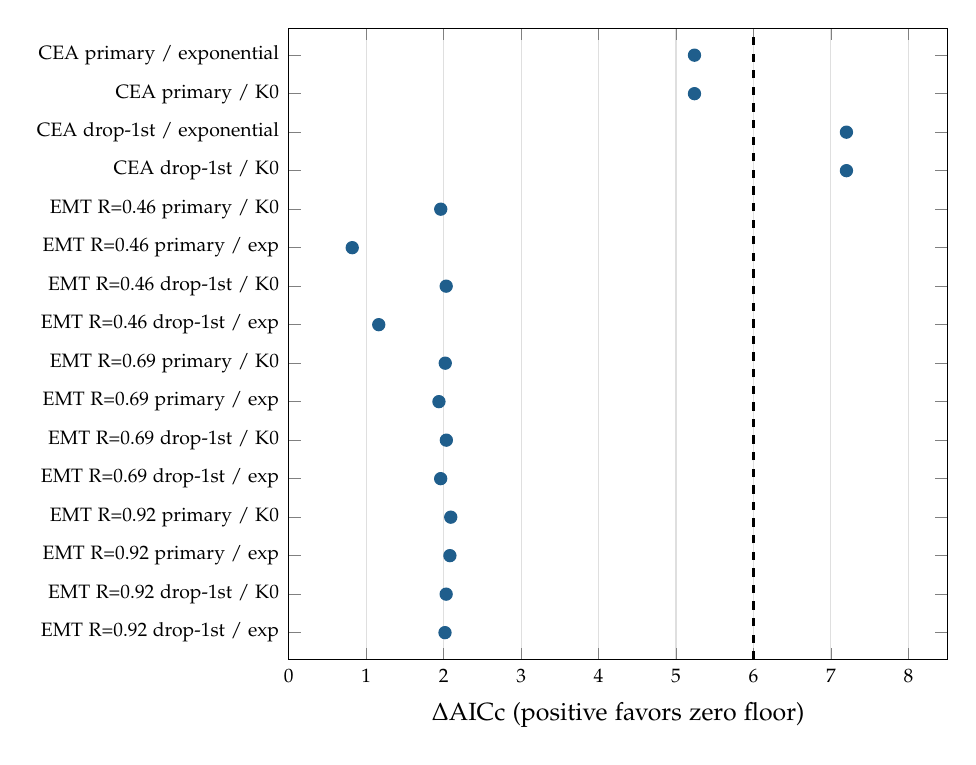
\begin{tikzpicture}
\begin{axis}[width=0.82\textwidth,height=9.6cm,xlabel={$\Delta\mathrm{AICc}$ (positive favors zero floor)},xmin=0,xmax=8.5,ymin=-0.7,ymax=15.7,ytick={0,1,2,3,4,5,6,7,8,9,10,11,12,13,14,15},yticklabels={{EMT R=0.92 drop-1st / exp},{EMT R=0.92 drop-1st / K0},{EMT R=0.92 primary / exp},{EMT R=0.92 primary / K0},{EMT R=0.69 drop-1st / exp},{EMT R=0.69 drop-1st / K0},{EMT R=0.69 primary / exp},{EMT R=0.69 primary / K0},{EMT R=0.46 drop-1st / exp},{EMT R=0.46 drop-1st / K0},{EMT R=0.46 primary / exp},{EMT R=0.46 primary / K0},{CEA drop-1st / K0},{CEA drop-1st / exponential},{CEA primary / K0},{CEA primary / exponential}},yticklabel style={font=\scriptsize},tick label style={font=\scriptsize},label style={font=\small},xmajorgrids=true,grid style={gray!25}]
\addplot[only marks,mark=*,mark size=2.2pt,accA] coordinates {(2.0170,0) (2.0322,1) (2.0805,2) (2.0915,3) (1.9613,4) (2.0344,5) (1.9389,6) (2.0203,7) (1.1619,8) (2.0324,9) (0.8194,10) (1.9623,11) (7.2000,12) (7.2000,13) (5.2381,14) (5.2381,15)};
\addplot[dashed,thick,black] coordinates {(6,-0.7)(6,15.7)};
\end{axis}
\end{tikzpicture}
\caption{Zero-floor versus positive-floor model competition ($\Delta\mathrm{AICc}>0$ favors the zero floor). Dashed line: the frozen decisive threshold $|\Delta\mathrm{AICc}|=6$. Only the CEA drop-first sensitivity crosses it; all EMT-I entries (three source separations, primary and drop-first tails, two families) lie below it, so the data there neither exclude nor establish a positive floor.}\label{fig:aicc}
\end{figure}

\subsection{Synthesis and falsification audit}\label{ssec:synth2}
The Stage~2 synthesis is \texttt{NO-\allowbreak{}UNIVERSAL-\allowbreak{}STRUCTURAL-\allowbreak{}EXCLUSION-\allowbreak{}DETECTED}, with the structural interpretation \texttt{STRUCTURAL-\allowbreak{}VACUUM-\allowbreak{}ACCESSIBILITY-\allowbreak{}SUPPORTED}. Concretely: (1) vacuum-directed behavior survives the move from connected field profiles to a vacuum-subtracted continuum EMT; (2) the EMT result survives the change of source separation without a floor; (3) ordered structural architecture is preserved across the CEA refinements even where absolute amplitude agreement fails; (4) the same architecture appears in the unsmoothed Battelli control; (5) no frozen primary or secondary branch returns a robust \texttt{ISOLATION-\allowbreak{}SUPPORTED}, \texttt{EMT-\allowbreak{}POSITIVE-\allowbreak{}FLOOR}, or equivalent positive-floor result. \Cref{tab:F} records the outcome of the seven preregistered failure modes.

\begin{table}[t]
\centering\small
\caption{Stage~2 falsification audit (F1--F7), as recorded in the Stage~2 synthesis.}\label{tab:F}
\begin{tabularx}{\textwidth}{@{}l>{\raggedright\arraybackslash}X>{\raggedright\arraybackslash}p{4.4cm}@{}}
\toprule
& Failure criterion & Outcome\\\midrule
F1 & Every admissible refinement path terminates before vacuum approach & Not observed (CEA and EMT contain vacuum-directed paths over their measured domains)\\
F2 & Common refinement produces $\Dstruct\ge\delta>0$ & Not observed (no stable positive-floor verdict)\\
F3 & Apparent approach disappears under independent representations & Not observed\\
F4 & Approach requires loss of admissibility & Not observed in the structural chambers used; not proved for all possible representations\\
F5 & Effect produced only by digitization, interpolation or window choice & Not supported (Baker downgraded; EMT needs no interpolation)\\
F6 & Continuity-like behavior only in synthetic controls & Not observed (measured lattice and published continuum profiles)\\
F7 & An independent structural chamber reproduces universal non-crossability & Not observed\\\bottomrule
\end{tabularx}
\end{table}

\paragraph{What Stage~2 has not established.} It does not prove $V\in\overline{\AYM}$. It has not delivered, with decisive precision, a single fully refinement-stable measured-data sequence $L_n\in\AYM$ with $\Dstruct(L_n,V)\to0$ under a representation-independent metric: the strongest primary CEA branch is \texttt{REFINEMENT-\allowbreak{}INDETERMINATE} and the primary EMT branch \texttt{EMT-\allowbreak{}UNCERTAINTY-\allowbreak{}LIMITED}. The absence of a detected floor is, in those branches, absence of decisive evidence for or against one; the support for accessibility comes from the convergence of branches and representations, not from any single decisive test. This is exactly the distinction between $\Hacc^{\rm emp}$ (supported) and $\Hacc^{\rm lim}$ (not established) of \cref{eq:status}.

%==============================================================
\section{Stage 3: independent spectral discreteness}\label{sec:stage3}

Stage~3 asks a different question of independent data: is there a strictly positive spectral scale for the lowest scalar excitation of pure SU(3) gauge theory? The stage was deliberately designed so that the structural and spectral sides stay independent: the structural side is carried forward unchanged from Stage~2, and the spectral side is established independently from continuum glueball spectroscopy. The target is not a numerical relation between them but coexistence. Two continuum anchors were frozen, each in its \emph{native coordinate}, and deliberately not converted into one another.

\subsection{SPEC-I/A: Athenodorou--Teper}
The continuum $0^{++}$ ground state in units of the string tension, taken from \cite{AT20}, is
\begin{equation}
\frac{M_{0^{++}}}{\sqs}=3.405(21),
\end{equation}
with the alternate source-supplied extrapolation $3.391(23)$ and lower one-sigma bounds $3.384$ and $3.368$; the frozen status is \texttt{SPECTRAL-\allowbreak{}SCALE-\allowbreak{}POSITIVE}. The underlying ladder of eight ensembles ($a\sqs=0.3999\to0.1038$) has $M/\sqs$ rising from $2.468(42)$ to $3.346(23)$, positive at every level (\cref{fig:spec}, left; \cref{tab:ladder}). These are lattice values, not continuum-extrapolated, shown only to display the approach to the continuum anchor. For context, \cref{tab:cont} lists the other channels from the same source; only the $A_1^{++}$ ground state enters the verdict.

\subsection{SPEC-I/B: Chen et al.}
In the independent anisotropic-lattice study \cite{Chen06} (five coupling values) the scalar glueball mass is
\begin{equation}
r_0 M_{0^{++}}=4.16(11)(4)
\end{equation}
(statistical and anisotropy errors). The preregistered conservative bound subtracts the two uncertainties linearly, $4.16-0.11-0.04=4.01>0$; the frozen status is \texttt{SPECTRAL-\allowbreak{}SCALE-\allowbreak{}POSITIVE}. A historical source value $4.21(11)$ was recorded as a check and \emph{not} counted as an independent Stage~3 branch.

\subsection{Independence and the refusal to convert}
The two anchors use different actions, scale conventions ($\sqs$ versus the Sommer parameter $r_0$ \cite{Sommer94}) and collaborations. We do not convert between $\sqs$ and $r_0$ merely to display agreement: independence is part of the argument, and each scale is positive in its own coordinate (\cref{fig:spec}, right). Forcing the two onto a common axis would add an assumption (a value of $r_0\sqs$) that neither source needs.

\begin{figure}[t]
\centering
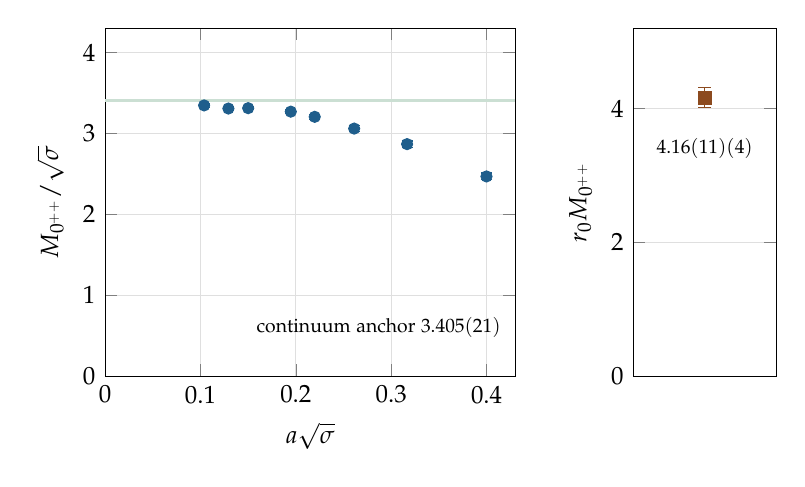
\begin{tikzpicture}
\begin{axis}[name=L,width=0.56\textwidth,height=6cm,xlabel={$a\sqrt{\sigma}$},ylabel={$M_{0^{++}}/\sqrt{\sigma}$},xmin=0,xmax=0.43,xtick={0,0.1,0.2,0.3,0.4},ymin=0,ymax=4.3,grid=major,grid style={gray!25},tick label style={font=\small},label style={font=\small}]
\fill[accC!25] (axis cs:0,3.384) rectangle (axis cs:0.43,3.426);
\addplot[only marks,mark=*,mark size=2pt,accA,error bars/.cd,y dir=both,y explicit] table[row sep=\\,x index=0,y index=1,y error index=2] {
0.39990 2.4681 0.0423\\
0.31666 2.8674 0.0384\\
0.26118 3.0596 0.0355\\
0.21982 3.2049 0.0316\\
0.19472 3.2688 0.0239\\
0.15003 3.3120 0.0204\\
0.12928 3.3075 0.0294\\
0.10383 3.3459 0.0226\\
};
\node[font=\scriptsize,anchor=south east] at (axis cs:0.425,0.35) {continuum anchor $3.405(21)$};
\end{axis}
\begin{axis}[at={(L.east)},xshift=1.5cm,anchor=west,width=0.28\textwidth,height=6cm,ylabel={$r_0M_{0^{++}}$},xmin=0,xmax=2,xtick=\empty,ymin=0,ymax=5.2,grid=major,grid style={gray!25},tick label style={font=\small},label style={font=\small}]
\addplot[only marks,mark=square*,mark size=2.4pt,accB,error bars/.cd,y dir=both,y explicit] coordinates {(1,4.16) +- (0,0.15)};
\node[font=\scriptsize,anchor=north] at (axis cs:1,3.7) {$4.16(11)(4)$};
\end{axis}
\end{tikzpicture}
\caption{Spectral positivity in native coordinates. \emph{Left:} Athenodorou--Teper lattice $M_{0^{++}}/\sqs$ against $a\sqs$ (error bars as recorded), with the continuum anchor $3.405(21)$ as a dashed line. \emph{Right:} the Chen et al.\ anchor $r_0M_{0^{++}}=4.16$ with its combined statistical-plus-anisotropy bar ($0.11+0.04$ added linearly). The panels use different coordinates and are not to be compared on one axis.}\label{fig:spec}
\end{figure}

\begin{table}[t]
\centering\small
\caption{Continuum glueball masses in units of $\sqs$ extracted from \cite{AT20} (Table~14 of the source); only the first row enters SPEC-I/A.}\label{tab:cont}
\begin{tabular}{@{}llc@{}}\toprule Channel & State & $M/\sqs$\\\midrule
$A1^{++}$ & ground & $3.405(21)$\\
$A1^{++}$ & first excitation & $5.855(41)$\\
$E^{++}$ & ground & $4.904(20)$\\
$T2^{++}$ & ground & $4.884(19)$\\
$A1^{-+}$ & ground & $5.276(45)$\\
\bottomrule\end{tabular}
\end{table}

%==============================================================
\section{BRIDGE-III: coexistence rather than identification}\label{sec:bridge}

BRIDGE-III is a deterministic evaluator over \emph{frozen statuses only}: it reads the Stage~2 status and the two SPEC-I statuses, verifies six checks, and emits an outcome; it does not rerun any chamber, refit any profile, alter any spectral number, or modify Stage~2. Its inputs and result are
\[
\begin{aligned}
&\texttt{STRUCTURAL-\allowbreak{}VACUUM-\allowbreak{}ACCESSIBILITY-\allowbreak{}SUPPORTED}\ \ (\text{Stage 2})\\
&\quad\wedge\ \texttt{SPECTRAL-\allowbreak{}SCALE-\allowbreak{}POSITIVE}\ (\text{SPEC-I/A})\ \wedge\ \texttt{SPECTRAL-\allowbreak{}SCALE-\allowbreak{}POSITIVE}\ (\text{SPEC-I/B})\\
&\quad\Longrightarrow\ \texttt{COEXISTENCE-\allowbreak{}SUPPORTED}.
\end{aligned}
\]
All six deterministic checks passed (structural status found; SPEC-I/A and SPEC-I/B statuses found; both numeric guards; theory match to pure SU(3)), and the three input files matched their recorded SHA-256 digests (\cref{app:repro}). The record states that earlier verdicts were not modified and that neither a mass-gap theorem nor a closure theorem is claimed. The project-level frozen result is \texttt{STRUCTURAL-\allowbreak{}SPECTRAL-\allowbreak{}COEXISTENCE-\allowbreak{}SUPPORTED}: within the frozen pure-SU(3) evidence architecture, structural accessibility is supported and coexists with spectral discreteness. Because the structural input is $\Hacc^{\rm emp}$, the coexistence claim is likewise empirical; it is not the limit statement $\Hacc^{\rm lim}$.

\begin{table}[t]
\centering\small
\caption{Margin of the frozen spectral scales above zero, each in its own native coordinate. Lower bounds are those recorded in the SPEC-I extracts (one-sigma for A; conservative linear for B).}\label{tab:margin}
\begin{tabular}{@{}llccc@{}}
\toprule
Branch & Coordinate & Central value & Lower bound & Central value $/\,\sigma$\\\midrule
SPEC-I/A & $M_{0^{++}}/\sqs$ & $3.405$ & $3.384$ & $3.405/0.021\approx162$\\
SPEC-I/B & $r_0M_{0^{++}}$ & $4.16$ & $4.01$ & $4.16/0.117\approx36$\\\bottomrule
\end{tabular}
\end{table}
(The last column divides the central value by the recorded one-sigma uncertainty, with $\sigma_B=\sqrt{0.11^2+0.04^2}\approx0.117$ used for provenance only.) Both scales are many standard deviations from zero; the point of Stage~3, however, is not the size of the margin but that positivity is retained independently of the structural stage.

\subsection{Master table of frozen verdicts}\label{sec:master}
\Cref{tab:master} condenses every frozen verdict and stage status of both projects with what each rules in and out; the exhaustive record with the representation tested and the question asked is in \cref{app:record}.

{\footnotesize
\setlength{\tabcolsep}{3pt}
\begin{longtable}{@{}l>{\raggedright\arraybackslash}p{3.3cm}>{\raggedright\arraybackslash}p{4.7cm}>{\raggedright\arraybackslash}p{6.4cm}@{}}
\caption{Master table of frozen verdicts (condensed from \cref{tab:verdicts}). G = \texttt{UNNS\_YM\_GAP}, V = \texttt{UNNS\_VACUUM\_CONTINUITY}.}\label{tab:master}\\
\toprule ID & Source & Verdict & Rules in / out\\\midrule\endfirsthead
\toprule ID & Source & Verdict & Rules in / out\\\midrule\endhead
\bottomrule\endfoot
G1 & \texttt{UNNS\_YM\_GAP}\ YM-0 & complete for the present program & In: preregistered protocol. Out: any physical claim.\\[2pt]
G2 & \texttt{UNNS\_YM\_GAP}\ YM-1 & sufficient for current work & In: data base for YM-2/3. Out: nothing physical.\\[2pt]
G3 & \texttt{UNNS\_YM\_GAP}\ YM-2A / STRUC-I & vacuum-compressed branch not rejected & Out: short ladder as non-crossability evidence.\\[2pt]
G4 & \texttt{UNNS\_YM\_GAP}\ YM-2A / STRUC-PERC-I & directionality test failed; representation/test pair falsified & Out: connectivity collapse $\equiv$ vacuum non-crossability.\\[2pt]
G5 & \texttt{UNNS\_YM\_GAP}\ YM-2B & \texttt{VACUUM-\allowbreak{}BOUNDARY DIAGNOSTIC ESTABLISHED; REFINEMENT TEST REQUIRED} (provisional) & In: fixed-resolution separation. Out: refinement stability.\\[2pt]
G6 & \texttt{UNNS\_YM\_GAP}\ YM-3A & \texttt{MODEL-\allowbreak{}REFINEMENT PERSISTENT} & In: model-family persistence. Out: measured-correlator persistence.\\[2pt]
G7 & \texttt{UNNS\_YM\_GAP}\ YM-3B & \texttt{DATA-\allowbreak{}INDETERMINATE} & In: central crossing at $\beta=6.71$. Out: stable falsification; stable persistence.\\[2pt]
G8 & \texttt{UNNS\_YM\_GAP}\ YM-4 & not entered / cancelled & Out: any structural-to-Hamiltonian bridge.\\[2pt]
G9 & \texttt{UNNS\_YM\_GAP}\ closure & \texttt{NOT ESTABLISHED} & Out: universal non-crossability as established; not a proof of its negation.\\[2pt]
\midrule
V0 & \texttt{UNNS\_VACUUM\_\allowbreak CONTINUITY}\ Stage 1 & FROZEN (definitions; no empirical verdict) & Out: ``basin\textquotedblright{}, ``attractor\textquotedblright{}, ``fixed point\textquotedblright{}.\\[2pt]
V1 & Baker 2022 \cite{Baker22}\ VREF-I/A & \texttt{CALIBRATION-\allowbreak{}SENSITIVE} & In: methodological warning. Out: continuity or isolation verdict.\\[2pt]
V2 & CEA 2017 \cite{Cea17}\ VREF-I/B & \texttt{REFINEMENT-\allowbreak{}INDETERMINATE} & In: vacuum-directed path, no floor detected. Out: absolute refinement-stable calibration; isolation.\\[2pt]
V3 & CEA 2017\ STRUC bridge & \texttt{ARCHITECTURE-\allowbreak{}PRESERVED} & In: structural organization stable. Out: absolute-amplitude agreement.\\[2pt]
V4 & Battelli 2019 \cite{Battelli19}\ control & \texttt{UNSMOOTHED-\allowbreak{}ARCHITECTURE-\allowbreak{}CONSISTENT} & In: corroboration. Out: independent primary distance measurement.\\[2pt]
V5 & Yanagihara 2019 \cite{Yanagihara19}\ EMT-I, $R=0.69$\,fm & \texttt{EMT-\allowbreak{}UNCERTAINTY-\allowbreak{}LIMITED} & In: vacuum-directed, zero floor favored numerically. Out: decisive floor exclusion; \texttt{EMT-\allowbreak{}CONTINUITY-\allowbreak{}CONSISTENT}.\\[2pt]
V6 & Yanagihara 2019\ geometry & \texttt{GEOMETRY-\allowbreak{}ROBUST-\allowbreak{}NO-\allowbreak{}FLOOR} & In: no floor at any tested separation. Out: floor-free proof.\\[2pt]
V7 & Stage 2 synthesis & \texttt{NO-\allowbreak{}UNIVERSAL-\allowbreak{}STRUCTURAL-\allowbreak{}EXCLUSION-\allowbreak{}DETECTED} & Out: universal non-crossability in tested representations.\\[2pt]
V8 & Stage 2 interpretation & \texttt{STRUCTURAL-\allowbreak{}VACUUM-\allowbreak{}ACCESSIBILITY-\allowbreak{}SUPPORTED} & In: accessibility (empirical). Out: $V\in\overline{\AYM}$ as a theorem.\\[2pt]
V9 & SPEC-I/A: AT20 \cite{AT20} & \texttt{SPECTRAL-\allowbreak{}SCALE-\allowbreak{}POSITIVE} & In: $\dspec>0$ in $\sqs$ units. Out: any structural statement.\\[2pt]
V10 & SPEC-I/B: Chen et al.\ \cite{Chen06} & \texttt{SPECTRAL-\allowbreak{}SCALE-\allowbreak{}POSITIVE} & In: independent positivity. Out: conversion between $\sqs$ and $r_0$.\\[2pt]
V11 & BRIDGE-III & \texttt{COEXISTENCE-\allowbreak{}SUPPORTED} & In: coexistence. Out: identification; mass-gap or closure theorem.\\[2pt]
V12 & Stage 3 / project & \texttt{STRUCTURAL-\allowbreak{}SPECTRAL-\allowbreak{}COEXISTENCE-\allowbreak{}SUPPORTED} & In: structural continuity can coexist with spectral discreteness (within frozen architecture). Out: Clay problem.\\[2pt]
\end{longtable}}


%==============================================================
\section{Discussion}\label{sec:discussion}

\subsection{Four notions of nearness}\label{ssec:four}
The original program asked a single question---is the vacuum surrounded by a structurally empty neighborhood?---but the word \emph{near} was carrying four different meanings. Separating them is, we think, the main conceptual gain of the whole exercise, and it is what turns the theorem of \cref{sec:theorem} from an appended remark into the organizing statement of the paper.

\paragraph{Configuration-space nearness.} Two field configurations are near if some metric on the configuration (or ensemble) space is small. This is the notion implicit in the phrase ``approaching the vacuum'' for a gauge field, and it is the one least accessible to our instruments: none of the frozen chambers operates on configurations. No representation-independent metric on $\AYM$ was constructed here.

\paragraph{Observable-space nearness.} Two states are near if a chosen family of gauge-invariant observables takes nearby values. All Stage~2 evidence lives here: the vacuum-subtracted chromoelectric profile, the energy-density tail, the four-component EMT norm. The statement ``no positive floor detected'' is a statement about this notion in five specific representations (\cref{ssec:synth2}). Observable-space nearness is representation-dependent by construction, which is why the structural chambers were required to agree across representations rather than within one.

\paragraph{Hilbert-space nearness.} Two states are near if their vectors in the physical Hilbert space are close in norm. The vacuum is the unique ground state, and states $\psi_\theta=\cos\theta\,\Omega+\sin\theta\,\varphi$ with $\varphi\perp\Omega$ converge to $\Omega$ in norm as $\theta\to0$. This notion is complete and canonical, but it is a property of the quantized theory and is not measured by any lattice profile directly. \Cref{ex:hilbert} shows what is at stake: along such a norm-convergent sequence a support-edge functional can stay at a fixed positive value, so Hilbert-space nearness does not by itself force energy nearness either.

\paragraph{Spectral nearness.} Two states are near if their energies are close, i.e.\ $\dspec(E_n,E_0)=|E_n-E_0|\to0$. A positive gap $\Delta=E_1-E_0$ is the statement that spectral nearness to $E_0$ is impossible for any state orthogonal to the vacuum. This is the only notion in which a gap has an unconditional meaning.

\begin{figure}[t]
\centering
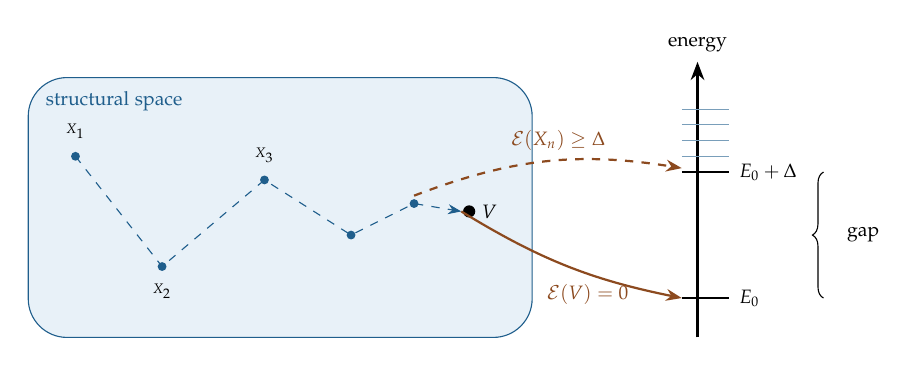
\begin{tikzpicture}[ar/.style={-{Stealth[length=2mm]},thick},>=Stealth]
\draw[rounded corners=14pt,fill=lvE,draw=accA] (-0.2,-1.6) rectangle (6.2,1.7);
\node[font=\scriptsize,anchor=north west,text=accA] at (-0.1,1.65) {structural space};
\fill (5.4,0) circle (2.2pt) node[right=1pt,font=\scriptsize] {$V$};
\foreach \x/\y/\n in {0.4/0.7/1,1.5/-0.7/2,2.8/0.4/3,3.9/-0.3/4,4.7/0.1/5}{\fill[accA] (\x,\y) circle (1.6pt);}
\node[font=\tiny,anchor=south] at (0.4,0.8) {$X_1$}; \node[font=\tiny,anchor=north] at (1.5,-0.8) {$X_2$}; \node[font=\tiny,anchor=south] at (2.8,0.5) {$X_3$};
\draw[accA,->,dashed] (0.4,0.7)--(1.5,-0.7)--(2.8,0.4)--(3.9,-0.3)--(4.7,0.1)--(5.3,0);
\draw[->,thick] (8.3,-1.6)--(8.3,1.9) node[above,font=\scriptsize] {energy};
\draw[thick] (8.1,-1.1)--(8.7,-1.1) node[right,font=\scriptsize] {$E_0$};
\draw[thick] (8.1,0.5)--(8.7,0.5) node[right,font=\scriptsize] {$E_0+\Delta$};
\draw[decorate,decoration={brace,amplitude=4pt}] (9.9,-1.1)--(9.9,0.5) node[midway,right=5pt,font=\scriptsize] {gap};
\foreach \y in {0.7,0.9,1.1,1.3}{\draw[accA!60] (8.1,\y)--(8.7,\y);}
\draw[ar,accB] (5.3,0) to[bend right=10] node[below,font=\scriptsize,pos=0.6] {$\mathcal E(V)=0$} (8.1,-1.1);
\draw[ar,accB,dashed] (4.7,0.2) to[bend left=15] node[above,font=\scriptsize,pos=0.55] {$\mathcal E(X_n)\ge\Delta$} (8.1,0.55);
\end{tikzpicture}
\caption{Schematic of the separation (not data). \emph{Left:} a structural space in which a sequence $X_n$ converges to $V$ ($D_{\rm struct}\to0$). \emph{Right:} the energy axis, with the vacuum level $E_0$ and a gap $\Delta$. The map $\mathcal E=E-E_0$ along the sequence jumps from $0$ at $V$ to a value $\ge\Delta$ at every $X_n$: the sequence is structurally convergent but spectrally separated. This is the situation of \cref{thm:sep}(a),(c); nothing here asserts that Yang--Mills realizes it.}\label{fig:top}
\end{figure}

\paragraph{What the theorem says about the four.} Convergence in the first three notions does not imply convergence in the fourth unless the map from the first three to energies is continuous at the vacuum. \Cref{thm:sep}(b) states that such continuity is a \emph{sufficient} bridge to an exclusion neighborhood; \cref{thm:sep}(c) states that accessibility under a persistent gap forces the oscillation of $\mathcal E$ at $V$ to be at least $\Delta$; and \cref{thm:sep}(d) localizes the failure to one of two maps. In plain words, the original program tacitly assumed that being close to the vacuum in structure means being close in energy; the gap is a statement about the second and says nothing about the first.

\paragraph{The sentence that must not be over-read.} Theorem~1 establishes that structural convergence need not imply spectral convergence. The empirical results are compatible with this architecture and support structural accessibility, but do not establish the limiting sequence required to instantiate the theorem in Yang--Mills. In the notation of \cref{eq:Hemp,eq:Hlim}: $\Hacc^{\rm emp}$ is supported; $\Hacc^{\rm lim}$ is not established; the premise of the theorem is therefore not empirically instantiated (\cref{rem:premise}), and the coexistence claim of BRIDGE-III is empirical coexistence within a frozen architecture, not a demonstration that the abstract counterexample is realized by the theory.

\subsection{Three readings of the coexistence}\label{ssec:readings}
Suppose, for the sake of the discussion, that the empirical finding survives further tests: structure is accessible and the gap is positive. By \cref{thm:sep}(d), with the factorization $\mathcal E=\mathcal E_{\rm sp}\circ\Pi$ through $\Pi:\SUNNS\to\Yspec$, at least one of two maps fails to be continuous at the vacuum. Three readings are logically available, and they are not equivalent.

\begin{enumerate}[label=(R\arabic*)]
\item \textbf{$\Pi$ is discontinuous at $V$.} Structural neighbors of the vacuum are spectrally far away: the structure-to-spectrum map jumps. This is the literal content of the abstract counterexample and the reading most directly suggested by the phrase ``structurally accessible but spectrally separated''. It predicts that a faithful $\Pi$ built from gauge-invariant correlators would show a finite jump in the extracted spectral data as the structural distance goes to zero, at fixed physical scale.
\item \textbf{$\mathcal E_{\rm sp}$ is discontinuous at the vacuum point of $\Yspec$.} The map from spectral states to energies is the discontinuous one. This happens if the topology of $\Yspec$ is too weak (for instance, if it identifies states whose spectral measures differ only in their lowest support point). Then the discontinuity is a feature of how spectral states are topologized, not of the structure-to-spectrum map, and a different choice of $\Yspec$ could remove it. The Hilbert-space example (\cref{ex:hilbert}) is of this kind: the functional $\psi\mapsto$ (edge of the spectral support) is not norm-continuous at $\Omega$ along $\psi\perp\Omega$.
\item \textbf{The topology on the structural side is the issue.} What we call $D_{\rm struct}$ in the five representations may simply be too coarse: two states with small observable distance may be far in a finer structural topology that would also see the gap. In that case ``accessibility'' would be an artifact of the resolution of the representation, and a sufficiently fine structural topology would restore an exclusion neighborhood. The frozen design cannot exclude this reading; the representation-diversity argument of Stage~2 reduces but does not eliminate it.
\end{enumerate}

None of the three is selected by the present data. The point of the list is that they ask for \emph{different} work: (R1) asks for an explicit construction and computation of $\Pi$; (R2) asks for a choice of $\Yspec$ and a proof of continuity or discontinuity of the energy functional on it; (R3) asks for a structural metric that is demonstrably not coarser than the spectral one. We regard (R2) as the most tractable, because it is a question about functional analysis on spaces of spectral measures that can be formulated without lattice input, and (R3) as the most dangerous, because it would reduce the Stage~2 conclusion to a statement about resolution.

\subsection{Confinement, scale generation and the mass gap}\label{ssec:confinement}
The three terms in the title of this subsection are often run together and the frozen evidence touches them unequally.

\paragraph{Confinement.} The flux-tube profiles of Stage~2 are confinement-sector observables. We use only their \emph{vacuum-subtracted tail}, i.e.\ the statement that the field returns toward the vacuum value away from the flux tube, and we do not model the tube itself. Nothing here constrains the confinement mechanism.

\paragraph{Scale generation.} The spectral anchors are quoted in units of $\sqrt\sigma$ and $r_0$, two scales generated dynamically by the theory. That $M_{0^{++}}/\sqs\approx3.4$ and $r_0M_{0^{++}}\approx4.2$ are $O(1)$ numbers in these units is the standard lattice statement that the theory has a single scale; the present paper uses it only to say that a positive spectral scale is present in two independent normalizations, and does not convert between them.

\paragraph{Mass gap.} The Clay formulation asks for a rigorous construction of the quantum theory on $\mathbb R^4$ together with a positive lower bound on the spectrum of the Hamiltonian above the vacuum \cite{JaffeWitten}. The lattice glueball masses used here are strong numerical evidence for a positive scalar excitation scale in a lattice regularization continued to the continuum \cite{Teper98,MorningstarPeardon99,Chen06,LuciniTeperWenger04,AT20}; they are not a proof of the continuum gap, and they are used here only as an \emph{independent positive input} in Stage~3. The structural stage never touches the Hamiltonian. This is the sense in which the conclusion is ``coexistence'' and not ``derivation of the gap''.

\subsection{What each stage contributes and what it cannot}\label{ssec:contrib}
Reading the whole program backwards from the theorem is instructive. Stage~1 (the original program) contributes a falsified test and a surviving diagnostic: the CORR-I statistic separates massive from gapless controls at fixed resolution, and the refinement test is indeterminate on measured data. Stage~2 contributes a robust negative: no universal positive floor was detected across profile, tail, bridge, control and geometry variations. Stage~3 contributes a positive that is independent of the structure. The theorem contributes the logical remark that the three results are consistent only if the missing bridge is either absent or non-continuous, and it names the object ($\Pi$) that must be studied to decide which.

It is worth stating what \emph{would} be a different, stronger paper: one that (i) constructs $\Pi$ on a concrete class of states, (ii) proves $\Hacc^{\rm lim}$ in that class, and (iii) shows the energy functional is discontinuous. We do none of these. The paper established a consistent logical frame, a body of frozen empirical evidence organized by it, and a precisely stated open problem.

\subsection{Methodological lessons}\label{ssec:lessons}
Several lessons from the two projects bear on how such programs should be run, independent of the Yang--Mills application.

\begin{enumerate}[label=(M\arabic*)]
\item \textbf{Freeze before the scientific batch.} Every verdict string in \cref{tab:master} was defined with its decision rule before the data were examined, and no verdict was modified afterwards. The outcome that most deserves this protection is the uncomfortable one: $\beta=6.71$ in YM-3B crosses zero, and the preregistered label (\texttt{DATA-\allowbreak{}INDETERMINATE}) is what the frame forced rather than what a narrative would have preferred.
\item \textbf{Distinguish a falsified test from a falsified hypothesis.} STRUC-PERC-I falsified the \emph{representation/test pair} (the directionality test failed); it did not falsify non-crossability. Treating the first as the second would have been an over-reach in the opposite direction.
\item \textbf{Report model-family persistence and measured-data persistence separately.} A clean persistence on exactly-constructed controls (Class C) says nothing about whether the same separation survives noise, reconstruction error and finite statistics (Class B). The gap between the two classes is where the original program stalled.
\item \textbf{Prefer cross-representation agreement to within-representation precision.} The positive result of Stage~2 does not come from any single fit; it comes from the same qualitative outcome in five different observables, none of which was constructed to produce it.
\item \textbf{Keep numerical preference and decisive exclusion apart.} Zero-floor models are numerically favored in the EMT sector ($\Delta\mathrm{AICc}\approx1.9$--$2.1$ at the primary geometry), but the frozen decisive threshold is $6$; the verdict is correspondingly \texttt{EMT-\allowbreak{}UNCERTAINTY-\allowbreak{}LIMITED}. Only the CEA drop-first sensitivity (7.200) crosses the threshold, and a sensitivity analysis is not allowed to promote the primary verdict.
\item \textbf{Separate admissibility from distance.} A profile can approach the vacuum proxy and still fail admission; VREF-I keeps the two checks apart so that the structural distance cannot be inflated by inadmissible inputs.
\end{enumerate}

%==============================================================
\section{Implications and the specialization problem}\label{sec:implications}

\subsection{The \texorpdfstring{$\Pi$}{Pi} problem}\label{ssec:pi}
The specialization of the theorem to Yang--Mills is the construction of the structure-to-spectrum map $\Pi:\SUNNS\to\Yspec$, where $\Yspec$ is a topological space of spectral states. A minimal requirement list follows from \cref{sec:theorem}.

\begin{enumerate}[label=(P\arabic*)]
\item \textbf{A concrete $\SUNNS$.} A class of structural states closed enough that $D_{\rm struct}$ is a genuine (pseudo)metric rather than a chamber-specific score, and in which the vacuum $V$ is a point whose neighborhoods can be discussed.
\item \textbf{A concrete $\Yspec$.} A space of spectral data---for instance positive spectral measures $\nu$ on $[0,\infty)$ representing Euclidean correlators $C(t)=\int e^{-Et}d\nu(E)$ \cite{OS73,OS75,GlimmJaffe}---equipped with a stated topology (weak-$*$, total variation, or a Hausdorff-moment topology \cite{ShohatTamarkin,Akhiezer}). The choice decides whether the energy functional $\mathcal E_{\rm sp}(\nu)=\inf(\mathrm{supp}\,\nu\setminus\{E_0\})-E_0$ is continuous: it is lower semicontinuous but not continuous in the weak topology, which is exactly the delicacy of (R2).
\item \textbf{A definition of $\Pi$ on gauge-invariant correlators.} The correlator chamber CORR-I is a first concrete step: it maps a Euclidean correlator to a positivity/contraction diagnostic. It is not yet a map into $\Yspec$.
\item \textbf{A statement of what is held fixed.} Physical volume, resolution, and scale-setting (\cite{Sommer94,LuscherWolff90}) must be specified in the definition of the limit; the present work only compares at matched physical scale.
\end{enumerate}

\subsection{A testable quantitative form}\label{ssec:holder}
Part (e) of \cref{thm:sep} gives a quantitative bridge: if $\mathcal E$ is $\alpha$-H\"older with constant $C$ near the vacuum, structural distance $\delta=\min\{r,(\Delta/C)^{1/\alpha}\}$ is excluded. For the program this is more useful than an abstract statement, because it turns the question into a number to be measured. If a family of structural states $X_n$ were produced with $D_{\rm struct}(X_n,V)\to0$ and a measured $\mathcal E(X_n)$, then
\[
\widehat C_\alpha=\sup_n \frac{\mathcal E(X_n)}{D_{\rm struct}(X_n,V)^{\alpha}}
\]
estimated from the data would either stay bounded (a H\"older bridge, hence an exclusion radius $\delta$) or diverge (failure of every H\"older bridge, hence accessibility with a gap). This is a falsifiable form of the dichotomy, and it requires exactly the sequence $\Hacc^{\rm lim}$ that the present evidence does not provide.

\subsection{Consequences for the original hypothesis}\label{ssec:consequences}
The original hypothesis $\Hiso$ remains \texttt{NOT ESTABLISHED}. The pivot does not refute it; it identifies it with a strong bridge assumption and observes that no evidence in either project supports that bridge. Two directions follow. If a continuity or H\"older bridge can be justified on independent grounds for a specified $\Pi$, $\Hiso$ would follow from the gap by \cref{thm:sep}(b),(e). If the bridge can be shown to fail, $\Hacc^{\rm lim}$ becomes the correct statement and the coexistence is real. The two outcomes are exclusive and both are informative.

\subsection{Outside Yang--Mills}\label{ssec:outside}
The theorem is not specific to gauge theory. Any system in which a structural distance and a spectral distance are defined independently---a lattice model, a quantum graph, a family of operators on a varying domain---is subject to the same dichotomy. The separation of nearness notions may therefore be useful as a checklist in other contexts in which a claim of the form ``proximity in one space implies proximity in another'' is made implicitly.

%==============================================================
\section{Limitations and falsifiability}\label{sec:limits}

\subsection{Limitations}\label{ssec:limitations}
\begin{enumerate}[label=(L\arabic*)]
\item \textbf{Elementary theorem.} \Cref{thm:sep} is essentially continuity. It is stated and proved for completeness and to locate the missing assumption, not as a deep result.
\item \textbf{Premise not instantiated.} $\Hacc^{\rm lim}$ is not established; neither is a representation-independent $D_{\rm struct}$.
\item \textbf{Profile windows, not excitations.} The Stage~2 states are windows of a vacuum-subtracted profile along the radial coordinate, not excitation sequences in a Hilbert space. The natural reading of Stage~2 is therefore about observable-space nearness (\cref{ssec:four}).
\item \textbf{Class B reconstruction.} The YM-3B inputs are digitized from published figures and reconstructed into proxies; the preregistered uncertainty procedure accounts for the reconstruction but cannot account for what the published figures omit.
\item \textbf{Smoothing and gradient flow.} Smeared and flowed observables suppress short-distance structure by design; the unsmoothed Battelli control reduces but does not eliminate this concern.
\item \textbf{Frozen architecture.} The coexistence claim is conditional on the frozen decision rules, thresholds (such as the decisive $|\Delta\mathrm{AICc}|\ge6$) and the choice of five representations. A different, equally reasonable architecture might produce different verdicts.
\item \textbf{Two spectral anchors.} SPEC-I/A and SPEC-I/B give two independent positive scales, but they are both lattice results; neither is a constructive-QFT bound.
\item \textbf{No Clay claim.} The present work does not construct the continuum theory, does not prove a gap, and does not prove $V\in\overline{\AYM\setminus\{V\}}$.
\end{enumerate}

\subsection{What would change the conclusions}\label{ssec:falsifiers}
The program is stated so that specific outcomes would force revision.
\begin{itemize}
\item A representation in which the vacuum-subtracted structural distance saturates at a positive floor, reproduced across refinements and across independent data, would falsify the \emph{universality} in \texttt{NO-\allowbreak{}UNIVERSAL-\allowbreak{}STRUCTURAL-\allowbreak{}EXCLUSION-\allowbreak{}DETECTED} (not the Stage~2 results in the other representations).
\item A decisive AICc preference ($\Delta\mathrm{AICc}\le-6$) for a positive floor in an admissible EMT dataset would convert \texttt{EMT-\allowbreak{}UNCERTAINTY-\allowbreak{}LIMITED} to a floor-supported verdict.
\item A refinement-stable Class B result for CORR-I (the sign of $S_B$ preserved at every level with the preregistered interval excluding zero) would promote the original diagnostic and revive the case for the original hypothesis.
\item A proof that $\Pi$ is continuous at $V$ for a physically motivated $\Yspec$, together with a gap, would imply an exclusion neighborhood by \cref{thm:sep}(b) and contradict $\Hacc^{\rm lim}$.
\item A measured continuum scalar mass compatible with zero in either normalization would void Stage~3.
\end{itemize}

%==============================================================
\section{Conclusion}\label{sec:conclusion}
We began with a hypothesis that the Yang--Mills mass gap forces a structurally non-crossable neighborhood around the vacuum. The program built to test it separated massive from gapless correlator controls at fixed resolution but did not establish refinement-stable non-crossability on measured data: the central verdict is \texttt{NOT ESTABLISHED}. Testing the complementary hypothesis---that the vacuum is structurally accessible---across five representations produced no universal positive exclusion floor, and two independent lattice results retain a strictly positive scalar scale. The combined, frozen result is \texttt{STRUCTURAL-\allowbreak{}SPECTRAL-\allowbreak{}COEXISTENCE-\allowbreak{}SUPPORTED}, an empirical statement within the frozen architecture.

The theorem proved here explains why this is not a contradiction: a spectral gap constrains energies, not structure, and the two are linked only by a bridge that the original program had assumed. Continuity at the vacuum is a sufficient bridge to structural exclusion; accessibility under a persistent gap forces that continuity to fail; and the failure localizes in either the structure-to-spectrum map or the topology of the spectral space. What remains is the hard specialization: to construct $\Pi:\SUNNS\to\Yspec$ for Yang--Mills, to establish the limit statement $\Hacc^{\rm lim}$ rather than the empirical $\Hacc^{\rm emp}$, and to determine the topology that decides the question. We state this as the open problem of the program, at Level~3 of the three-level separation (\cref{sec:intro}), and make no claim about the Clay problem.

%==============================================================
\appendix
\section{Exhaustive verdict record}\label{app:record}
\Cref{tab:verdicts} lists every frozen verdict and stage status of both projects, with the representation tested, the question asked, and what the verdict rules in and out.

\begin{landscape}
{\footnotesize
\setlength{\tabcolsep}{4pt}
\begin{longtable}{@{}l>{\raggedright\arraybackslash}p{3.3cm}>{\raggedright\arraybackslash}p{3.8cm}>{\raggedright\arraybackslash}p{4.4cm}>{\raggedright\arraybackslash}p{4.6cm}>{\raggedright\arraybackslash}p{5.2cm}@{}}
\caption{Every frozen verdict and stage status of \texttt{UNNS\_YM\_GAP} (G) and \texttt{UNNS\_VACUUM\_CONTINUITY} (V). Verdict strings are quoted exactly as frozen.}\label{tab:verdicts}\\
\toprule ID & Source & Representation & Question & Verdict & Rules in / out\\\midrule\endfirsthead
\toprule ID & Source & Representation & Question & Verdict & Rules in / out\\\midrule\endhead
\bottomrule\endfoot
G1 & \texttt{UNNS\_YM\_GAP}\ YM-0 & Formalization & Frozen hypotheses, observables, null rules, refinement logic, falsification criteria & complete for the present program & In: preregistered protocol. Out: any physical claim.\\[3pt]
G2 & \texttt{UNNS\_YM\_GAP}\ YM-1 & Gauge-invariant glueball/lattice corpus & Is there a working corpus of gauge-invariant quantities? & sufficient for current work & In: data base for YM-2/3. Out: nothing physical.\\[3pt]
G3 & \texttt{UNNS\_YM\_GAP}\ YM-2A / STRUC-I & Six-node vacuum-anchored spectral ladder & Does vacuum compression (gap reduced up to $\times1024$) leave the ladder inadmissible? & vacuum-compressed branch not rejected & Out: short ladder as non-crossability evidence.\\[3pt]
G4 & \texttt{UNNS\_YM\_GAP}\ YM-2A / STRUC-PERC-I & Same ladder, four deformation families & Is fragmentation specific to approach toward the vacuum? & directionality test failed; representation/test pair falsified & Out: connectivity collapse $\equiv$ vacuum non-crossability.\\[3pt]
G5 & \texttt{UNNS\_YM\_GAP}\ YM-2B & CORR-I correlator chamber (AT20) & Does $R_{\rm contract}$ separate massive from gapless adversaries at fixed resolution? & \texttt{VACUUM-\allowbreak{}BOUNDARY DIAGNOSTIC ESTABLISHED; REFINEMENT TEST REQUIRED} (provisional) & In: fixed-resolution separation. Out: refinement stability.\\[3pt]
G6 & \texttt{UNNS\_YM\_GAP}\ YM-3A & Class C mass-anchored controls, 8 levels & Does the separation persist under common refinement? & \texttt{MODEL-\allowbreak{}REFINEMENT PERSISTENT} & In: model-family persistence. Out: measured-correlator persistence.\\[3pt]
G7 & \texttt{UNNS\_YM\_GAP}\ YM-3B & Class B Sakai--Sasaki reconstruction, 4 levels & Does the separation persist for measured data? & \texttt{DATA-\allowbreak{}INDETERMINATE} & In: central crossing at $\beta=6.71$. Out: stable falsification; stable persistence.\\[3pt]
G8 & \texttt{UNNS\_YM\_GAP}\ YM-4 & Bridge theorem under original premise & --- & not entered / cancelled & Out: any structural-to-Hamiltonian bridge.\\[3pt]
G9 & \texttt{UNNS\_YM\_GAP}\ closure & Whole project & Is a refinement-stable non-crossable vacuum boundary established? & \texttt{NOT ESTABLISHED} & Out: universal non-crossability as established; not a proof of its negation.\\[3pt]
\midrule
V0 & \texttt{UNNS\_VACUUM\_\allowbreak CONTINUITY}\ Stage 1 & Ontology $V\in\overline{\AYM\setminus\{V\}}$; VREF-I & What is meant by ``vacuum belongs to the substrate\textquotedblright{}; failure criteria F1--F7 & FROZEN (definitions; no empirical verdict) & Out: ``basin\textquotedblright{}, ``attractor\textquotedblright{}, ``fixed point\textquotedblright{}.\\[3pt]
\midrule
V1 & Baker 2022 \cite{Baker22}\ VREF-I/A & Common-refinement profiles, 3 resolutions & Is the refinement ordering interpolation-independent? & \texttt{CALIBRATION-\allowbreak{}SENSITIVE} & In: methodological warning. Out: continuity or isolation verdict.\\[3pt]
V2 & CEA 2017 \cite{Cea17}\ VREF-I/B & Connected field profile, deep tail & Zero floor vs positive floor; cross-refinement agreement & \texttt{REFINEMENT-\allowbreak{}INDETERMINATE} & In: vacuum-directed path, no floor detected. Out: absolute refinement-stable calibration; isolation.\\[3pt]
V3 & CEA 2017\ STRUC bridge & STRUC-I / STRUC-PERC-I on 5 ladders & Does refinement change regime or topology? & \texttt{ARCHITECTURE-\allowbreak{}PRESERVED} & In: structural organization stable. Out: absolute-amplitude agreement.\\[3pt]
V4 & Battelli 2019 \cite{Battelli19}\ control & Unsmoothed connected correlator, 3 ladders & Is the architecture an artifact of smearing? & \texttt{UNSMOOTHED-\allowbreak{}ARCHITECTURE-\allowbreak{}CONSISTENT} & In: corroboration. Out: independent primary distance measurement.\\[3pt]
V5 & Yanagihara 2019 \cite{Yanagihara19}\ EMT-I, $R=0.69$\,fm & Vacuum-subtracted 4-component EMT norm & Zero floor vs positive floor (decisive $|\Delta$AICc$|\ge6$) & \texttt{EMT-\allowbreak{}UNCERTAINTY-\allowbreak{}LIMITED} & In: vacuum-directed, zero floor favored numerically. Out: decisive floor exclusion; \texttt{EMT-\allowbreak{}CONTINUITY-\allowbreak{}CONSISTENT}.\\[3pt]
V6 & Yanagihara 2019\ geometry & Same at $R=0.46,\,0.92$\,fm & Is the result geometry-dependent? & \texttt{GEOMETRY-\allowbreak{}ROBUST-\allowbreak{}NO-\allowbreak{}FLOOR} & In: no floor at any tested separation. Out: floor-free proof.\\[3pt]
V7 & Stage 2 synthesis & All Stage 2 branches & Is a universal refinement-stable positive floor detected? & \texttt{NO-\allowbreak{}UNIVERSAL-\allowbreak{}STRUCTURAL-\allowbreak{}EXCLUSION-\allowbreak{}DETECTED} & Out: universal non-crossability in tested representations.\\[3pt]
V8 & Stage 2 interpretation & Same & What does V7 support? & \texttt{STRUCTURAL-\allowbreak{}VACUUM-\allowbreak{}ACCESSIBILITY-\allowbreak{}SUPPORTED} & In: accessibility (empirical). Out: $V\in\overline{\AYM}$ as a theorem.\\[3pt]
V9 & SPEC-I/A: AT20 \cite{AT20} & $M_{0^{++}}/\sqs=3.405(21)$ & Is the continuum scalar scale positive? & \texttt{SPECTRAL-\allowbreak{}SCALE-\allowbreak{}POSITIVE} & In: $\dspec>0$ in $\sqs$ units. Out: any structural statement.\\[3pt]
V10 & SPEC-I/B: Chen et al.\ \cite{Chen06} & $r_0M_{0^{++}}=4.16(11)(4)$ & Same, independent source and scale & \texttt{SPECTRAL-\allowbreak{}SCALE-\allowbreak{}POSITIVE} & In: independent positivity. Out: conversion between $\sqs$ and $r_0$.\\[3pt]
V11 & BRIDGE-III & Frozen statuses V8, V9, V10 & Do accessibility and spectral positivity coexist? & \texttt{COEXISTENCE-\allowbreak{}SUPPORTED} & In: coexistence. Out: identification; mass-gap or closure theorem.\\[3pt]
V12 & Stage 3 / project & Whole project & Project-level result & \texttt{STRUCTURAL-\allowbreak{}SPECTRAL-\allowbreak{}COEXISTENCE-\allowbreak{}SUPPORTED} & In: structural continuity can coexist with spectral discreteness (within frozen architecture). Out: Clay problem.\\[3pt]
\end{longtable}}
\end{landscape}


\section{Supporting data}\label{app:data}
\subsection{YM-3A: Class C eight-level refinement}
\begin{table}[ht]\centering\small\caption{YM-3A primary common-grid results (all matched orderings pass).}\label{tab:ym3a}
\begin{tabular}{@{}rcccc@{}}\toprule $\beta$ & $R_{\rm massive}$ & $R_{p=8}$ matched & $S_{\rm fixed}$ & $S_{\rm match}$\\\midrule
5.6924 & 0.018556 & 0.041575 & 0.708018 & 0.806712\\
5.8 & 0.012377 & 0.040156 & 1.112950 & 1.176904\\
5.8941 & 0.010214 & 0.039234 & 1.305025 & 1.345755\\
5.99 & 0.008840 & 0.038463 & 1.449513 & 1.470402\\
6.0625 & 0.008297 & 0.038108 & 1.512884 & 1.524494\\
6.235 & 0.007950 & 0.037863 & 1.555686 & 1.560841\\
6.338 & 0.007985 & 0.037888 & 1.551275 & 1.557102\\
6.5 & 0.007688 & 0.037668 & 1.589194 & 1.589194\\
\bottomrule\end{tabular}\end{table}
\subsection{YM-3B: Class B four-level refinement}
\begin{table}[ht]\centering\small\caption{YM-3B central results and preregistered sensitivity.}\label{tab:ym3b}
\begin{tabular}{@{}rcccccc@{}}\toprule $\beta$ & $R_B$ & $R_{p=8}$ & $S_B$ & $S_B^{\rm PCHIP}$ & 95\% interval & matched order\\\midrule
6.2 & 0.088576 & 0.092825 & 0.020350 & 0.019648 & [0.004053, 0.035659] & pass\\
6.4 & 0.082775 & 0.089902 & 0.035867 & 0.036198 & [0.017167, 0.053094] & pass\\
6.71 & 0.092700 & 0.091978 & $-$0.003395 & $-$0.003948 & [$-$0.027454, 0.019320] & fail\\
6.93 & 0.082333 & 0.092774 & 0.051851 & 0.052060 & [0.024726, 0.081194] & pass\\
\bottomrule\end{tabular}\end{table}
\noindent Nested ladder lengths (L5/L6/L7) at $\beta=6.71$: $S_B=-0.007663,\,-0.006666,\,-0.003395$; at the other three $\beta$ all lengths are positive.
\subsection{Baker calibration windows}
\begin{table}[ht]\centering\small\caption{Ratio $C=R_{23}/R_{12}$ of successive refinement distances by window and interpolation.}
\begin{tabular}{@{}ccccc@{}}\toprule window & $[u_0,u_1]$ & $C_{\rm linear}$ & $C_{\rm PCHIP}$ & class (lin/PCHIP)\\\midrule
0 & [0, 0.5] & 0.449 & 0.357 & $<$1 / $<$1\\
1 & [0.125, 0.625] & 0.546 & 0.275 & $<$1 / $<$1\\
2 & [0.25, 0.75] & 0.532 & 0.544 & $<$1 / $<$1\\
3 & [0.375, 0.875] & 0.987 & 1.036 & $<$1 / $>$1\\
4 & [0.5, 1] & 1.485 & 1.529 & $>$1 / $>$1\\
\bottomrule\end{tabular}\end{table}
\subsection{CEA refinement mismatch}
\begin{table}[ht]\centering\small\caption{CEA tail amplitude of the two physical refinements (R1, R2 common-linear), $\mathrm{GeV}^2$ as recorded.}
\begin{tabular}{@{}cccc@{}}\toprule $x$ (fm) & $E_{R1}$ & $E_{R2}$ & $E_{R2}/E_{R1}$\\\midrule
0.381 & 0.1242 & 0.1330 & 1.071\\
0.476 & 0.0726 & 0.0810 & 1.116\\
0.571 & 0.0409 & 0.0466 & 1.137\\
0.666 & 0.0222 & 0.0258 & 1.161\\
0.761 & 0.0117 & 0.0139 & 1.184\\
\bottomrule\end{tabular}\end{table}
\subsection{AT20 lattice ladder}
\begin{table}[ht]\centering\small\caption{Eight AT20 ensembles: $A_1^{++}$ ground-state mass in lattice units and in $\sqs$ units.}\label{tab:ladder}
\begin{tabular}{@{}rccccc@{}}\toprule level & $\beta$ & lattice & $a\sqs$ & $aM$ & $M/\sqs$\\\midrule
1 & 5.6924 & $10^3\times 16$ & 0.39990 & 0.9870(90) & 2.468(42)\\
2 & 5.8 & $12^3\times 16$ & 0.31666 & 0.9080(120) & 2.867(38)\\
3 & 5.8941 & $14^3\times 16$ & 0.26118 & 0.7991(92) & 3.060(35)\\
4 & 5.99 & $18^3\times 18$ & 0.21982 & 0.7045(65) & 3.205(32)\\
5 & 6.0625 & $20^3\times 20$ & 0.19472 & 0.6365(43) & 3.269(24)\\
6 & 6.235 & $26^3\times 26$ & 0.15003 & 0.4969(29) & 3.312(20)\\
7 & 6.338 & $30^3\times 30$ & 0.12928 & 0.4276(37) & 3.308(29)\\
8 & 6.5 & $38^3\times 38$ & 0.10383 & 0.3474(22) & 3.346(23)\\
\bottomrule\end{tabular}\end{table}


\section{Reproducibility and provenance}\label{app:repro}
\noindent All structural and spectral inputs of this paper are the frozen records of the two projects; no number was re-fitted for the paper. The analytics page built from the same records verified 21 verdict strings and audited the frozen-manifest hashes below. SHA-256 digests:

\begin{tabular}{@{}>{\raggedright\arraybackslash}p{4.4cm}l@{}}\toprule Item & SHA-256\\\midrule
CORR-I v0.1.2 chamber & \texttt{\scriptsize f972c9d460cebc19ef165e66c03f971411062eba093876406ed2efe614e2deb2}\\
BRIDGE-III input \texttt{STAGE2\_STATUS.md} & \texttt{\scriptsize 991476088907af31c6d0256a992f79780e51eeef9e163d006e50ea4246e16582} \\
BRIDGE-III input \texttt{SPEC\_I\_A\_RESULT.md} & \texttt{\scriptsize 3d0d60dd827fdc953c684d8eaca0b8b9bd7d9ac14763d321a8bc39465972ba54} \\
BRIDGE-III input \texttt{SPEC\_I\_B\_RESULT.md} & \texttt{\scriptsize 0318aa14e92058facab9aa2527d1a4f34bc846400453f0f67ade0b5fd8be6caf} \\
Chen06 source PDF & \texttt{\scriptsize 66973cf81063071cf5c58d93cff86d4778b7d8f11e83eb1f3b89a21be3047f22}\\
AT20 published (SPEC-I/A) & \texttt{\scriptsize af40f084cf4f4624224af726d0bb4822e449b161b03ce38972077023cbd0ca7c}\\
AT20 arXiv v2 (SPEC-I/A) & \texttt{\scriptsize f0eb6406bf49a00d376c0be25917173426c826050046a1bf0f32987895de23d0}\\
\bottomrule\end{tabular}

\medskip
\noindent Frozen-manifest audit: 9 of 9 Stage~2 manifest entries matched their recorded digests; BRIDGE-III's three input digests matched (\cref{sec:bridge}). BRIDGE-III run timestamp (UTC): 2026-10-05T22:43:34.


%==============================================================
\begin{thebibliography}{99}\small
\bibitem{JaffeWitten} A.~Jaffe and E.~Witten, ``Quantum Yang--Mills theory,'' in \emph{The Millennium Prize Problems}, Clay Mathematics Institute (2006), official problem description.
\bibitem{Wilson74} K.~G.~Wilson, ``Confinement of quarks,'' Phys.\ Rev.\ D \textbf{10} (1974) 2445.
\bibitem{Creutz80} M.~Creutz, ``Monte Carlo study of quantized SU(2) gauge theory,'' Phys.\ Rev.\ D \textbf{21} (1980) 2308.
\bibitem{GattringerLang} C.~Gattringer and C.~B.~Lang, \emph{Quantum Chromodynamics on the Lattice}, Lecture Notes in Physics \textbf{788}, Springer (2010).
\bibitem{Teper98} M.~J.~Teper, ``Glueball masses and other physical properties of SU(N) gauge theories in D=3+1: a review of lattice results for theorists,'' arXiv:hep-th/9812187.
\bibitem{MorningstarPeardon99} C.~J.~Morningstar and M.~Peardon, ``The glueball spectrum from an anisotropic lattice study,'' Phys.\ Rev.\ D \textbf{60} (1999) 034509.
\bibitem{LuciniTeperWenger04} B.~Lucini, M.~Teper and U.~Wenger, ``Glueballs and k-strings in SU(N) gauge theories: calculations with improved operators,'' JHEP \textbf{06} (2004) 012.
\bibitem{Chen06} Y.~Chen \emph{et al.}, ``Glueball spectrum and matrix elements on anisotropic lattices,'' Phys.\ Rev.\ D \textbf{73} (2006) 014516, arXiv:hep-lat/0510074.
\bibitem{AT20} A.~Athenodorou and M.~Teper, ``The glueball spectrum of SU(3) gauge theory in 3+1 dimensions,'' JHEP \textbf{11} (2020) 172, arXiv:2007.06422.
\bibitem{SS23} K.~Sakai and S.~Sasaki, ``Glueball spectroscopy in lattice QCD using gradient flow,'' Phys.\ Rev.\ D \textbf{107} (2023) 034510, arXiv:2211.15176.
\bibitem{Sommer94} R.~Sommer, ``A new way to set the energy scale in lattice gauge theories and its application to the static force and $\alpha_s$ in SU(2) Yang--Mills theory,'' Nucl.\ Phys.\ B \textbf{411} (1994) 839.
\bibitem{Bali01} G.~S.~Bali, ``QCD forces and heavy quark bound states,'' Phys.\ Rept.\ \textbf{343} (2001) 1.
\bibitem{Greensite03} J.~Greensite, ``The confinement problem in lattice gauge theory,'' Prog.\ Part.\ Nucl.\ Phys.\ \textbf{51} (2003) 1.
\bibitem{Cea17} P.~Cea, L.~Cosmai, F.~Cuteri and A.~Papa, ``Flux tubes in the QCD vacuum,'' Phys.\ Rev.\ D \textbf{95} (2017) 114511, arXiv:1702.06437.
\bibitem{Baker22} M.~Baker, V.~Chelnokov, L.~Cosmai, F.~Cuteri and A.~Papa, ``Unveiling confinement in pure gauge SU(3): flux tubes, fields, and magnetic currents,'' arXiv:2207.08797.
\bibitem{Battelli19} N.~Battelli and C.~Bonati, ``Color flux tubes in SU(3) Yang--Mills theory: An investigation with the connected correlator,'' Phys.\ Rev.\ D \textbf{99} (2019) 114501, arXiv:1903.10463.
\bibitem{Yanagihara19} R.~Yanagihara, T.~Iritani, M.~Kitazawa, M.~Asakawa and T.~Hatsuda, ``Distribution of stress tensor around static quark--anti-quark from Yang--Mills gradient flow,'' Phys.\ Lett.\ B \textbf{789} (2019) 210.
\bibitem{Luscher10} M.~L\"uscher, ``Properties and uses of the Wilson flow in lattice QCD,'' JHEP \textbf{08} (2010) 071.
\bibitem{Suzuki13} H.~Suzuki, ``Energy-momentum tensor from the Yang--Mills gradient flow,'' PTEP \textbf{2013} (2013) 083B03, arXiv:1304.0533.
\bibitem{LuscherWolff90} M.~L\"uscher and U.~Wolff, ``How to calculate the elastic scattering matrix in two-dimensional quantum field theories by numerical simulation,'' Nucl.\ Phys.\ B \textbf{339} (1990) 222.
\bibitem{OS73} K.~Osterwalder and R.~Schrader, ``Axioms for Euclidean Green's functions,'' Commun.\ Math.\ Phys.\ \textbf{31} (1973) 83.
\bibitem{OS75} K.~Osterwalder and R.~Schrader, ``Axioms for Euclidean Green's functions II,'' Commun.\ Math.\ Phys.\ \textbf{42} (1975) 281.
\bibitem{GlimmJaffe} J.~Glimm and A.~Jaffe, \emph{Quantum Physics: A Functional Integral Point of View}, 2nd ed., Springer (1987).
\bibitem{ShohatTamarkin} J.~A.~Shohat and J.~D.~Tamarkin, \emph{The Problem of Moments}, American Mathematical Society (1943).
\bibitem{Akhiezer} N.~I.~Akhiezer, \emph{The Classical Moment Problem}, Oliver \& Boyd (1965).
\bibitem{Akaike74} H.~Akaike, ``A new look at the statistical model identification,'' IEEE Trans.\ Automat.\ Control \textbf{19} (1974) 716.
\bibitem{HurvichTsai89} C.~M.~Hurvich and C.-L.~Tsai, ``Regression and time series model selection in small samples,'' Biometrika \textbf{76} (1989) 297.
\bibitem{BurnhamAnderson02} K.~P.~Burnham and D.~R.~Anderson, \emph{Model Selection and Multimodel Inference}, 2nd ed., Springer (2002).
\bibitem{FritschCarlson80} F.~N.~Fritsch and R.~E.~Carlson, ``Monotone piecewise cubic interpolation,'' SIAM J.\ Numer.\ Anal.\ \textbf{17} (1980) 238.
\end{thebibliography}
\end{document}
